\chapter{常微分方程$\frac{dy}{dx}=f(x,y)$的数值解法}
参考文献:《数值分析》(第4版)李庆扬 王能超 易大义 编,p336第9章 常微分方程初值问题数值解法

我们为什么要去解方程?因为方程是我们做的东西功能的抽象或者是自然规律的抽象,只有这样才方便我们具体分析,只有这样才具有普遍性,而不是一个特例,拿到别处就没用了。所以具体应用时,这个方程反映的就是我们系统,以$\frac{dy}{dx}=f(x,y)$为例,$x$通常表示是我们的输入,而输入是我们可以控制的,$y$是输出。我们很关心一个$x$的值(输入)对应$y$的值(输出)是多少。这也就说明了我们解方程的目的,目的就是找出$x$与$y$的关系,即,这个方程中自变量与应变量的关系。

这里我们先回顾下当初上第一堂课老师就讲的方程解的表示方法。有解析解,用一个函数就将所有的解抽象表示出来,这样的解当然是最理想的解,因为我想知道哪个$x$的值对应的$y$是多少,将$x$的值代进去算就知道了。但是实际上是很少能有具体的解析解。还有就是数值解,没有函数表达式,直接求出一系列的$x$的值对应的$y$值。而我们实际生活中真正关心的也是这些具体数值的对应。所以数值解法很实用。

初值问题
$$\begin{cases}\cfrac{dy}{dx}=f(x,y),&a\le x\le b\\ y(a)=c &\end{cases}$$
是常微分方程定解问题的最简单最常用的形式,这里讨论的就是它。参考资料:\cite{数值分析}p336第9章 常微分方程初值问题数值解法

\textbf{(1)数值解的存在唯一性}

只要函数$f(x,y)$适当光滑,例如,满足利普希茨(Lipschitz)条件
$$|f(x,y)-f(x,\tilde{y})|\le L|y-\tilde{y}|$$
理论上就可以保证上面初值问题的解$y=y(x)$存在并且唯一。

$L$是$f(x,y)$关于$y$的利普希茨常数。$L$的具体数值如何确定?

\textbf{(2)数值解法的思想}

所谓数值解法,就是寻求解$y(x)$在一系列离散节点
$$x_1<x_2<\cdots <x_n <x_{n+1}<\cdots$$
上的近似值
$$y_1,y_2,\cdots,y_n,y_{n+1},\cdots$$

相邻两个节点的间距$h_n=x_{n+1}-x_n$称为\textbf{步长}。今后如不特别说明,总是假定$h_i=h(i=1,2,\cdots)$为定数,这时节点为$x_n=x_0+nh,n=0,1,2,\cdots$。

这里的初值问题的数值解法有个基本特点,它们都采取“步进式”,即求解过程顺着节点排列的次序一步一步地向前推进。描述这类算法,只要给出用已知信息$y_n,y_{n-1},y_{n-2},\cdots$计算$y_{n+1}$的递推公式。

首先要对方程$\begin{cases}\cfrac{dy}{dx}=f(x,y),&a\le x\le b\\ y(a)=c &\end{cases}$离散化,建立求数值解的递推公式。一类是计算$y_{n+1}$时只用到前一点的值$y_n$,称为单步法。另一类是用到$y_{n+1}$前面$k$点的值$y_n,y_{n-1},\cdots,y_{n-k+1}$,称为$k$步法。其次,要研究公式的局部截断误差和阶,数值解$y_n$与精确解$y(x_n)$的误差估计及收敛性,还有递推公式的计算稳定性等问题。



\section{简单数值方法与基本概念}

\subsection{欧拉法}
$$\begin{cases}\cfrac{dy}{dx}=f(x,y),&a\le x\le b\\ y(a)=c &\end{cases}$$
的解是$y=y(x)$,$y=y(x)$在$xy$平面上是一条线。从几何观点看,$f(x,y)$则成了$y=y(x)$的斜率。已知初值$x_0,y_0$,由公式$f(x,y)$就可以求得$y=y(x)$在$(x_0,y_0)$点处的斜率。如图,


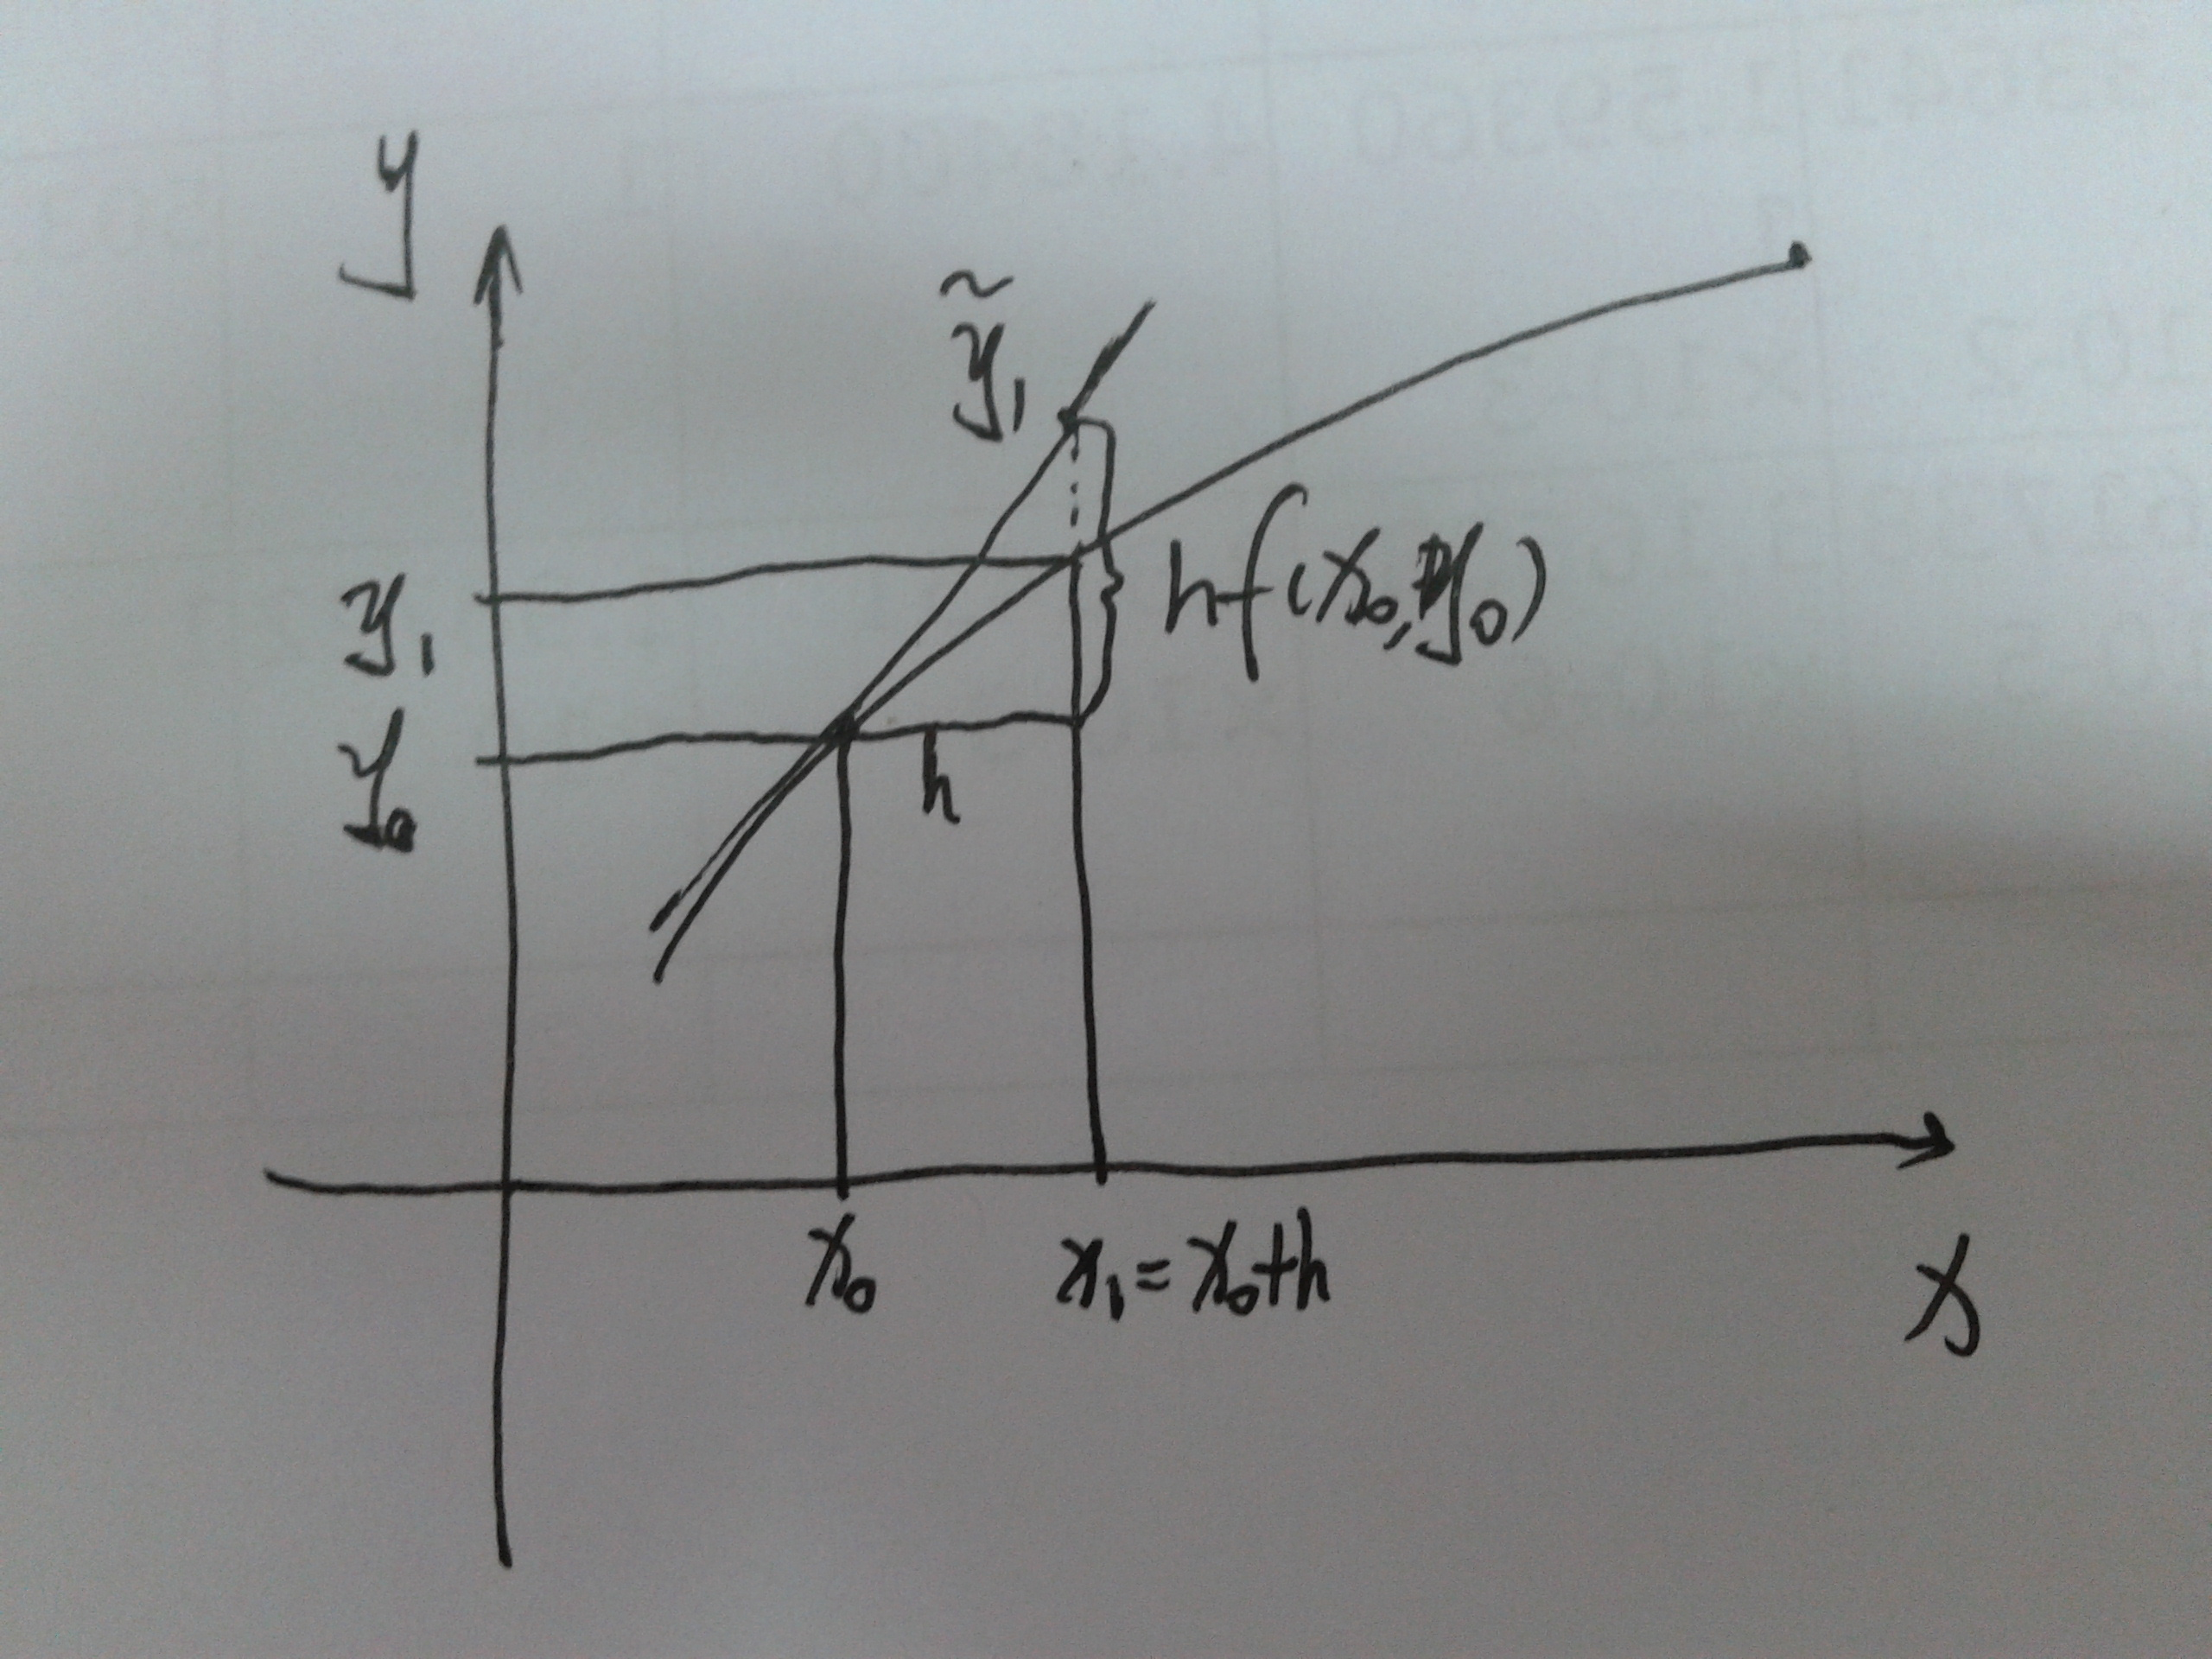
\includegraphics[width=0.7\textwidth]{pictures/2012-07-25.jpg}


有:
$$\tilde{y}_1=y_0+hf(x_0,y_0)\sim y_1$$
近似有:
$$y_{n+1}= y_n+h f(x_n,y_n)$$
这就是欧拉公式。

如果将步长$h$取的很小,与初始值相邻的第一个值$(x_1,y_1)$求得的近似值$(x_1,\tilde{y}_1)$可以说是非常精确的。但之后一的求解是将近似值$(x_1,\tilde{y}_1)$作为初始值进行计算,很明显,正在越来越偏离准确值,非常大的误差正在形成。这一点在后面的具体例子中可以明显看出。



\subsection{后退欧拉法(隐式)}
对$\frac{dy}{dx}=f(x,y)$从$x_n$到$x_{n+1}$积分,得
$$y(x_{n+1})=y(x_n)+\int_{x_n}^{x_{n+1}}f(t,y(t))dt$$
将右端的积分用右矩形公式$hF(x_{n+1},y(x_{n+1}))$代替,得
$$y_{n+1}=y_n+hf(x_{n+1},y_{n+1})$$
这个公式称为后退欧拉公式。

后退欧拉公式与欧拉公式有着本质的区别,欧拉公式是关于$y_{n+1}$的一个直接的计算公式,这类公式称作是\textbf{显式的}。后退欧拉公式右端含有未知的$y_{n+1}$,实际上是关于$y_{n+1}$的一个函数方程,这类公式称作是\textbf{隐式的}。

隐式方程通常用迭代法求解,而迭代过程的实质是逐步显式化。

\subsubsection{迭代法对后退欧拉公式求解}
\textbf{求解过程}

1、先用欧拉公式给出迭代初值$y_{n+1;0}$(前面已经说过,欧拉公式给出的第一个相邻值还是非常精确的)
$$y_{n+1;0}=y_n+hf(x_n,y_n)$$
其中下标中分号“;”后的数字表示迭代次数。

2、将迭代初值$y_{n+1;0}$代入后退欧拉公式
$$y_{n+1;1}=y_n+hf(x_{n+1},y_{n+1;0})$$


3、如此反复进行,得
$$y_{n+1;k+1}=y_n+hf(x_{n+1};y_{n+1;k}) \qquad (k=0,1,\cdots)$$

看到这个迭代过程,很容易产生一个问题:这样迭代求出的解是不是趋进于精确解,即是否收敛?下面就来讨论。



\textbf{解的收敛性}

由于$f(x,y)$对$y$满足利普希茨(Lipschitz)条件
$$|f(x,y)-f(x,\tilde{y})|\le L|y-\tilde{y}|$$
$L$是$f(x,y)$关于$y$的利普希茨常数。$L$的具体数值如何确定?

将$y_{n+1;k+1}=y_n+hf(x_{n+1};y_{n+1;k})$减去$y_{n+1}=y_n+hf(x_{n+1},y_{n+1})$即,将迭代$k$后的后退欧拉公式减去还未迭代的后退欧拉公式,有
$$|y_{n+1;k+1}-y_{n+1}|=h|f(x_{n+1},y_{n+1;k+1})-f(x_{n+1},y_{n+1})|
\le hL|y_{n+1,k}-y_{n+1}|$$
这个公式可以看出,只要$hL<1$,每次迭代出的解都比上一次迭代出的解趋近与精确解,即,后退欧拉法的迭代公式收敛到精确解。



\subsection{梯形公式(隐式)}
对$\frac{dy}{dx}=f(x,y)$从$x_n$到$x_{n+1}$积分,得
$$y(x_{n+1})=y(x_n)+\int_{x_n}^{x_{n+1}}f(t,y(t))dt$$
为了得到比后退欧拉法精度更高的计算公式,右端积分用梯形求积公式近似(梯形是比矩形更准确些)
$$y_{n+1}=y_n+\frac{h}{2}[f(x_n,y_n)+f(x_{n+1},y_{n+1})]$$
这个公式称为梯形公式。

梯形公式也是隐式的,也用迭代法求解,仍用欧拉公式提供迭代初值,其迭代公式为
$$\begin{cases}y_{n+1;0}=y_n+hf(x_n,y_n)\\
y_{n+1;k+1}=y_n+\frac{h}{2}[f(x_n,y_n)+f(x_{n+1},y_{n+1;k})]\\
(k=0,1,2\cdots)\end{cases}$$

梯形迭代公式解的收敛性讨论:

与后退欧拉公式迭代求解差不多,只不过这里是将未迭代的公式减去迭代$k$后的公式,
$$y_{n+1}-y_{n+1;k+1}=\frac{h}{2}[f(x_{n+1,y_{n+1}})-f(x_{n+1},y_{n+1;k})]$$
利用利普希茨条件$|f(x,y)-f(x,\tilde{y})|\le L|y-\tilde{y}|$,有
$$|y_{n+1}-y_{n+1;k+1}|\le \frac{hL}{2}|y_{n+1}-y_{n+1;k}|$$
由此可知,如果选取$h$充分小,使得$\frac{hL}{2}<1$,则当$k\rightarrow \infty$时,有$y_{n+1;k+1}\rightarrow y_{n+1}$,即梯形迭代公式是收敛的。



\subsection{改进欧拉法}
梯形方法虽然提高了精度,但其算法复杂,在应用梯形迭代公式进行实际计算时,没迭代一次,都要重新计算函数$f(x,y)$的值,而迭代又要反复进行若干次,计算量很大,而且往往难以预测。为了控制计算量,通常只迭代一两次就转入下一步的计算,这就简化了算法。

\textbf{思路如下:}

先用欧拉公式求得一个初步的近似值$\tilde{y}_{n+1}$,称之为\textbf{预测值}。预测值$\tilde{y}_{n+1}$的精度可能很差,在用梯形公式将它校正一次,即迭代一次得$y_{n+1}$,这个结果称为\textbf{校正值}。这样建立的预测-校正系统称为\textbf{改进的欧拉公式:}
\begin{align*}
&\text{预测}\qquad \tilde{y}_{n+1}=y_n+hf(x_n,y_n)=y_p\\
&\text{校正}\qquad y_{n+1}=y_n+\frac{h}{2}[f(x_n,y_n)+f(x_{n+1},\tilde{y}_{n+1})]
\end{align*}
即:
$$y_{n+1}=\frac{y_n}{2}+\frac{h}{2}f(x_n,y_n)+\frac{y_n}{2}+\frac{h}{2}f(x_{n+1};\tilde{y}_{n+1})$$
由此改写成平均化形式为
$$\begin{cases}
y_p = y_n+hf(x_n,y_n)\\
y_c = y_n+hf(x_{n+1},y_p)\\
y_{n+1}=\frac{1}{2}(y_p+y_c)
\end{cases}$$
其中$p$表示prediciton,$c$表示correction。




\subsection{单步法的局部截断误差与阶}
初值问题$\begin{cases}\cfrac{dy}{dx}=f(x,y),&a\le x\le b\\ y(a)=c &\end{cases}$单步法的一般形式为:
$$y_{n+1}=y_n+h\varphi(x_n,y_n,y_{n+1},h)$$
其中多元函数$\varphi$与$f(x,y)$有关。

当$\varphi$含有$y_{n+1}$时,方法是隐式的。若不含$y_{n+1}$则为显式方法,该\textbf{显式单步法}表示为:
$$y_{n+1}=y_n+h\varphi(x_n,y_n,h)$$
$\varphi(x,y,h)$称为增量函数,例如欧拉法有$\varphi(x,y,h)=f(x,y)$。

对一般显式单步法局部截断误差定义如下:

\textbf{定义1}

设$y(x)$是初值问题$\begin{cases}\cfrac{dy}{dx}=f(x,y),&a\le x\le b\\
y(a)=c &\end{cases}$的准确解,假设在$x_n$前各步没有误差,即$y_n$是准确解$y(x_n)$。$x_n$下一步的数值解为:$y_{n+1}=y_n+h\varphi(x_n,y_n,h)$,将精确解$y(x_{n+1})$减去数值解$y_{n+1}$就得到计算这步的误差:
$$T_{n+1}=y(x_{n+1})-y(x_n)-h\varphi(x_n,y(x_n),h)$$
$T_{n+1}$称为显式单步法$y_{n+1}=y_n+h\varphi(x_n,y_n,h)$的局部截断误差。从定义可以看出,$T_{n+1}$之所以称为局部截断误差是因为它反映的是显式单步法计算一步时的误差。

$T_{n+1}$的表达式是很好理解的,$y(x_{n+1})-y(x_n)$表示的是从$x_n$步到$x_{n+1}$精确解间的差值。而$h\varphi(x_n,y_n,h)$表示的是从$x_n$步到$x_{n+1}$数值解间的差值(前提假设是$x_n,y_n$是精确解,$x_n,y_n$可以理解为这步数值计算的初值)。由此这步精确解间的差值和这步数值解间的差值之差反映的当然是这步数值计算的误差,而反映的误差只限于这一步计算,故称为局部误差。

但是实际计算中$y_n$并不是精确解,这个误差定义也就是初值$x_0,y_0$的下一步$x_1,y_1$严格满足。……例子中算算步误差是否在这个误差定义的范围内……


\textbf{定义2}

设$y(x)$是初值问题$\begin{cases}\cfrac{dy}{dx}=f(x,y),&a\le x\le b\\y(a)=c &\end{cases}$的准确解,若存在最大整数$p$使显式单步法的局部截断误差满足
$$T_{n+1}=y(x+h)-y(x)-h\varphi(x,y,h)=O(h^{p+1})$$
则称显式单步法具有$p$阶精度。若将上式写成
$$T_{n+1}=\psi(x_n,y(x_n))h^{p+1}+O(h^{p+2})$$
则$\psi(x_n,y(x_n))h^{p+1}$称为局部截断误差主项。这样的形式对误差的表示是很有意义的,就$T_{n+1}$而言,其本身就是个小量,这个小量中,又存在更高阶的小量$O(h^{p+2})$,故实际讨论中,可以将这个更高阶小量$O(h^{p+2})$略去,余下的局部截断误差主项$\psi(x_n,y(x_n))h^{p+1}$已经就能很好的描述误差了。

\subsubsection{欧拉法的局部截断误差}
欧拉公式为:
$$y_{n+1}=y_n+hf(x_n,y_n)$$

利用定义1,有:
$$T_{n+1}=y(x_{n+1})-y(x_n)-hf(x_n,y(x_n))$$
将$y(x_{n+1})=y(x_n+h)$在$x_n$用泰勒展开:
\begin{align*}
y(x_{n+1})=y(x_n+h)&=y(x_n)+y\rq{}(x_n)(x_n+h-x_n)+\frac{y\rq{}\rq{}(x_n)}{2!}(x_n+h-x_n)^2+O(h^3)\\
&=y(x_n)+hy\rq{}(x_n)+\frac{h^2}{2}y\rq{}\rq{}(x_n)+O(h^3)
\end{align*}
将$f(x_n,y(x_n))$改写$y\rq{}(x_n)$\footnote{$f(x_n,y(x_n))$=$y\rq{}(x_n)$,$f(x,y)$就是$y(x)$的斜率,看原方程就知道了。},于是,有:
$$T_{n+1}=\frac{h^2}{2}y\rq{}\rq{}(x_n)+O(h^3)$$
根据定义2,局部截断误差主项为$\cfrac{\hbar^2}{2}y\rq{}\rq{}(x_n)$。就整个$T_{n+1}$而言,将高阶项$O(h^3)$略去($T_{n+1}$本来就是小量),则$T_{n+1}=O(h^2)$。根据定义$p=1$,即欧拉法是1阶方法。



\subsubsection{后退欧拉法局部截断误差}
后退欧拉公式为:
$$y_{n+1}=y_n+hf(x_{n+1},y_{n+1})$$

利用定义1,有:
$$T_{n+1}=y(x_{n+1})-y(x_n)-hf(x_{n+1},y(x_{n+1}))$$
将$y(x_{n+1})=y(x_n+h),f(x_{n+1},y(x_{n+1}))=y\rq{}(x_{n+1})=y\rq{}(x_n+h)$在$x_n$处泰勒展开,有:
\begin{align*}
y(x_{n+1})=y(x_n+h)&=y(x_n)+y\rq{}(x_n)(x_n+h-x_n)+\frac{y\rq{}\rq{}(x_n)}{2!}(x_n+h-x_n)^2+O(h^3)\\
&=y(x_n)+hy\rq{}(x_n)+\frac{h^2}{2}y\rq{}\rq{}(x_n)+O(h^3)
\end{align*}
\begin{align*}
f(x_{n+1},y(x_{n+1}))&=y\rq{}(x_{n+1})=y\rq{}(x_n+h)
=y\rq{}(x_n)+hy\rq{}\rq{}(x_n)+O(h^2)
\end{align*}
代入$T_{n+1}$中,有:
\begin{align*}
T_{n+1}&=y(x_n)+hy\rq{}(x_n)+\frac{h^2}{2}y\rq{}\rq{}(x_n)+O(h^3)
-y(x_n)-h[y\rq{}(x_n)+hy\rq{}\rq{}(x_n)+O(h^2)]\\
&=-\frac{h^2}{2}y\rq{}\rq{}(x_n)+O(h^3)
\end{align*}
这里$O(h^2)$直接抹去了,是因为有更高阶的小量$O(h^3)$在。

按照定义2,$p=1$,是1阶方法,局部截断误差主项为$-\cfrac{h^2}{2}y\rq{}\rq{}(x_n)$。



\subsubsection{梯形法局部截断误差}
梯形公式为:
$$y_{n+1}=y_n+\frac{h}{2}[f(x_n,y_n)+f(x_{n+1},y_{n+1})]$$
利用定义1,有:
$$T_{n+1}=y(x_{n+1})-y(x_n)-\frac{h}{2}[y\rq{}(x_n)+y\rq{}(x_{n+1})]$$
将$y(x_{n+1})=y(x_n+h),f(x_{n+1},y(x_{n+1}))=y\rq{}(x_{n+1})=y\rq{}(x_n+h)$在$x_n$处泰勒展开,有:
\begin{align*}
&y(x_n+h)=y(x_n)+hy\rq{}+h^2\frac{y\rq{}\rq{}(x_n)}{2!}+h^3\frac{y\rq{}\rq{}\rq{}(x_n)}{3!}+O(h^4)\\
&f(x_{n+1},y(x_{n+1}))=y\rq{}(x_{n+1})=y\rq{}(x_n+h)
=y\rq{}(x_n)+hy\rq{}\rq{}(x_n)+\frac{h^2}{2}y\rq{}\rq{}\rq{}(x_n)+O(h^3)
\end{align*}
这里为什么展开的级数和上面两个不一样,那是因为必须凑成定义2的形式,从上式看的到$y\rq{}(x_n),y\rq{}\rq{}(x_n)$都相消为0了。

代入$T_{n+1}$中,有:
\begin{align*}
T_{n+1}=&y(x_n)+hy\rq{}+h^2\frac{y\rq{}\rq{}(x_n)}{2!}+h^3\frac{y\rq{}\rq{}\rq{}(x_n)}{3!}+O(h^4)-y(x_n)\\
& -\frac{h}{2}[y\rq{}(x_n)+y\rq{}(x_n)+hy\rq{}\rq{}(x_n)+\frac{h^2}{2}y\rq{}\rq{}\rq{}(x_n)+O(h^3)]\\
=&\frac{h^3}{6}y\rq{}\rq{}\rq{}(x_n)-\frac{h^3}{4}y\rq{}\rq{}\rq{}(x_n)+O(h^3)\\
=&-\frac {h^3}{12}y\rq{}\rq{}\rq{}(x_n)+O(h^4)
\end{align*}
根据定义2,梯形法是二阶的,其局部误差主项为$-\cfrac {h^3}{12}y\rq{}\rq{}\rq{}(x_n)$。



\section{龙格—库塔法}
\subsection{显式龙格-库塔法的一般形式}
方程
$$\begin{cases}\cfrac{dy}{dx}=f(x,y),&a\le x\le b\\ y(a)=c &\end{cases}$$
等价积分形式为
$$y(x_{n+1})=y(x_n)+\int_{x_n}^{x_{n+1}}f(x,y(x))dx$$
若要是公式阶数提高,就必须使右端积分的数值求积公式精度提高,它必然要增加求积节点,为此将上式右端用求积公式表示为
$$\int_{x_n}^{x_{n+1}}f(x,y(x))dx\approx h\sum_{i=1}^r c_i f(x_n+\lambda_i h,y(x_n+\lambda_i h))$$
\textbf{这个公式应该是龙格库塔法思想的核心。}这个公式给人感觉是在由$x_n$到$x_{n+1}$步中又分出个$r$步计算,增加步数当然能提高精度了。

为了得到便于计算的显式方法,类似改进欧拉法
$$y_{n+1}=y_n+\frac{h}{2}[f(x_n,y_n)+f(x_n+h,y_n+hf(x_n,y_n))]$$

将$y_{n+1}$表示为
$$y_{n+1}=y_n+h\varphi(x_n,y_n,h)$$
其中
$$\varphi(x_n,y_n,h)=\sum_{i=1}^rc_iK_i,
\qquad K_1=f(x_n,y_n),
\qquad K_i=f(x_n+\lambda_i h, y_n+h\sum_{j=1}^{i-1}\mu_{ij}K_j)
\qquad i=2,\cdots,r$$
这里$c_i,\lambda_i,\mu_{ij}$均为常数。这个公式称为$r$级显式龙格-库塔法(Runge-Kutta),简称R-K法。

当$r=1$,$\varphi(x_n,y_n,h)=f(x_n,y_n)$,是欧拉法,此时方法的阶为$p=1$。



\subsection{二阶显式R-K法}
当$r=2$时,由$r$级显式龙格-库塔法,有
$$\begin{cases}y_{n+1}=y_n+h(c_1K_1+c_2K_2) \\
K_1=f(x_n,y_n)\\
K_2=f(x_n+\lambda_2h,y_n+\mu_{21}hK_1)
\end{cases}$$
这里$c_1,c_2,\lambda_2,\mu_{21}$均为待定常数,不同系数有不同表达式。可见改进欧拉法就是一种二阶显式龙格-库塔法。适当选取这些系数,是公式阶数$p$尽量高,通过局部截断误差来确定这些系数。

根据局部截断误差的定义,其局部截断误差为
$$T_{n+1}=y(x_{n+1})-y(x_n)-h[c_1f(x_n,y_n)+c_2f(x_n+\lambda_2h,y_n+\mu_{21}hf_n)]$$
其中$y_n=y(x_n),f_n=f(x_n,y_n)$。

为得到$T_{n+1}$的阶$p$,将上式各项在$(x_n,y_n)$处做泰勒展开\footnote{为什么不像后退欧拉法和梯形法,化成$y(x_n+h)$的形式,在$x_n$处泰勒展开?那是因为寻找处阶$p$的目标是化成局部截断误差定义2的形式,这里的项$f(x_n+\lambda_2h,y_n+\mu_{21}hf_n)$是没办法搞成这种形式。后退欧拉法和梯形法只需$y(x_n)$各级导数形式就达成这个目标了,不需要用$f(x_n,y_n)$二元泰勒展开,展开也是多此一举,会相消掉。},由于$f(x,y)$是二元函数,用二元泰勒展开,各项展开式为
\begin{align*}
y(x_{n+1}) = y(x_n+h)=y_n+hy\rq{}+\frac{h^2}{2}y\rq{}\rq{}_n+\frac{h^3}{3!}y\rq{}\rq{}\rq{}_n+O(h^4)
\end{align*}
其中
$$\begin{cases}
y\rq{}_n =f(x_n,y_n)=f_n\\
y\rq{}\rq{}_n=\frac{\partial}{\partial x}y\rq{}_n=\frac{\partial}{\partial x}f(x_n,y_n)=f\rq{}_x(x_n,y_n)+f\rq{}_y(x_n,y_n)\cdot y\rq{}_n=f\rq{}_x(x_n,y_n)+f\rq{}_y(x_n,y_n)\cdot f_n\\
y\rq{}\rq{}\rq{}_n=f\rq{}\rq{}_{xx}(x_n,y_n)+f\rq{}\rq{}_{xy}(x_n,y_n)y\rq{}_n
+f\rq{}\rq{}_{yx}(x_n,y_n)f_n+f^2_nf\rq{}\rq{}_{yy}(x_n,y_n)\\
\qquad\qquad+f\rq{}_y(x_n,y_n)[f\rq{}_x(x_n,y_n)+f\rq{}_y(x_n,y_n)\cdot f(x_n,y_n)]\\
\qquad =f\rq{}\rq{}_{xx}(x_n,y_n)+2f_nf\rq{}_{xy}(x_n,y_n)+f^2_nf\rq{}\rq{}_{yy}(x_n,y_n)+f\rq{}_y(x_n,y_n)[f\rq{}_x(x_n,y_n)+f_nf\rq{}_y(x_n,y_n)]
\end{cases}$$
注意推导时多次用到第一个式子$y\rq{}_n =f(x_n,y_n)=f_n$替换,还有$f\rq{}\rq{}_{xy}(x_n,y_n)$和$f\rq{}\rq{}_{yx}(x_n,y_n)$是相等的,求导顺序不影响结果。
\begin{align*}
f(x_n+\lambda_2h,y_n+\mu_21hf_n)
=f_n+f\rq{}_x(x_n,y_n)\lambda_2h+f\rq{}_y(x_n,y_n)\mu_{21}hf_n+O(h^2)
\end{align*}

观察$f(x_n+\lambda_2h,y_n+\mu_{21}hf_n)$发现$y(x_{n+1})$展开到4阶时,$y\rq{}\rq{}\rq{}_n$项中的$f\rq{}_yf\rq{}_x+f\rq{}_yf$不能通过选择参数消掉,也就说$r=2$的龙格-库塔公式不能使局部误差提高到$O(h^4)$。实际上要使$h^3$项为零,需增加3个方程,要确定4个参数$c1,c_1,\lambda_2$及$\mu_{21}$,这是不可能的。故$r=2$的显式龙格-库塔法的阶只能是$p=2$,而不能得到三阶公式。

$y(x_{n+1})$最多只能展开到2阶,即:
\begin{align*}
y(x_{n+1}) = y(x_n+h)=y_n+hy\rq{}+\frac{h^2}{2}y\rq{}\rq{}_n+O(h^3)
\end{align*}
代入到$T_{n+1}$,有
\begin{align*}
T_{n+1}=&y_n+hy\rq{}+\frac{h^2}{2}y\rq{}\rq{}_n+O(h^3)-y(x_n)\\
&-h\{c_1f(x_n,y_n)
+c_2[f_n+f\rq{}_x(x_n,y_n)\lambda_2h+f\rq{}_y(x_n,y_n)\mu_{21}hf_n+O(h^2)]\}\\
=&y_n+hf_n+\frac{h^2}{2}[f\rq{}_x(x_n,y_n)+f\rq{}_y(x_n,y_n)\cdot f_n]+O(h^3)-y(x_n)\\
&-h\{c_1f(x_n,y_n)
+c_2[f_n+f\rq{}_x(x_n,y_n)\lambda_2h+f\rq{}_y(x_n,y_n)\mu_{21}hf_n+O(h^2)]\}\\
=&(1-c_1-c_2)f_nh+\left(\frac{1}{2}-c_2\lambda_2\right)f\rq{}_x(x_n,y_n)h^2-\left(\frac{1}{2}-c_2\mu_{21}\right)f\rq{}_y(x_n,y_n)f_nh^2+O(h^3)
\end{align*}
要使$p=2$阶,必须使
$$1-c_1-c_2=0,\qquad \frac{1}{2}-c_2\lambda_2=0,\qquad \frac{1}{2}-c_2\mu_{21}=0$$
即
$$c_2\lambda_2=\frac{1}{2} ,\qquad c_2\mu_{21}=\frac{1}{2} ,\qquad c_1+c_2=1$$
它的解不是唯一的,令$c_2=a\ne 0$,则
$$c_1=1-a ,\qquad \lambda_2=\mu_{21}=\frac{1}{2a} $$
这样得到的公式称为二阶龙格-库塔法。

如果取$a=\frac{1}{2}$,则$c_1=c_2=\frac{1}{2} ,\lambda_2=\mu_{21}=1$,这就是改进欧拉法。

若取$a=1$,则$c_2=1,c_1=0,\lambda_2=\mu_{21}=\frac{1}{2}$,得到计算公式
$$\begin{cases}
y_{n+1}=y_n+hK_2\\
K_1=f(x_n,y_n)\\
K_2=f(x_n+\frac{h}{2},y_n+\frac{h}{2}K_1)
\end{cases}$$
称为中点公式,相当与数值积分的中矩形公式,也可以表示为
$$y_{n+1}=y_n+hf(x_n+\frac{h}{2},y_n+\frac{h}{2}f(x_n,y_n)$$



\subsection{三阶显式龙格-库塔法}
$r=3$可以得到三阶显式龙格-库塔法,其表达式为
$$\begin{cases}
y_{n+1}=y_n+h(c_1K_1+c_2K_2+c_3K_3)\\
K_1=f(x_n,y_n)\\
K_2=f(x_n+\lambda_2h,y_n+\mu_{21}hK_1)\\
K_3=f(x_n+\lambda_3h,y_n+\mu_{31}hK_1+\mu_{32}hK_2)
\end{cases}$$
其中$c_1,c_2,c_3$及$\lambda_2,\mu_{21},\lambda_3,\mu_{31},\mu_{32}$均为待定参数。该公式的局部截断误差为
$$T_{n+1}=y(x_{n+1})-y(x_n)-h[c_1K_1+c_2K_2+c_3K_3]$$
将$K_2,K_3$按二元函数泰勒展开,使$T_{n+1}=O(h^4)$,可得待定参数满足方程
$$\begin{cases}
c_1+c_2+c_3=1\\
\lambda_2=\mu_{21}\\
\lambda_3=\mu_{31}+\mu_{32}\\
c_2\lambda_2+c_3\lambda_3=\frac{1}{2}\\
c_2\lambda_2^2+c_3\lambda_3^2=\frac{1}{3}\\
c_3\lambda_2\mu_{32}=\frac{1}{6}
\end{cases}$$
这是8个未知数6个方程的方程组,解也不是唯一的,可以得到很多公式,这些公式统称为三阶龙格-库塔公式。

常见的三阶龙格-库塔公式为
$$\begin{cases}
y_{n+1}=y_n+\frac{h}{6}(K_1+4K_2+K_3)\\
K_1=f(x_n,y_n)\\
K_2=f(x_n+\frac{h}{2},y_n+\frac{h}{2}K_1)\\
K_3=f(x_n+h,y_n-hK_1+2hK_2)
\end{cases}$$



\subsection{四阶龙格-库塔法}
类似二阶、三阶龙格-库塔法推导过程可以推导出各种四阶龙格-库塔公式,常用公式为
$$\begin{cases}
y_{n+1}=y_n+\cfrac{h}{6}(K_1+2K_2+2K_3+K_4)\\
K_1=f(x_n,y_n)\\
K_2=f(x_n+\cfrac{h}{2},y_n+\cfrac{h}{2}K_1)\\
K_3=f(x_n+\cfrac{h}{2},y_n+\cfrac{h}{2}K_2)\\
K_4=f(x_n+h,y_n+hK_3)
\end{cases}
$$
其截断误差为$O(h^5)$。二阶的推导已经比较烦了,四阶推导可以想象有多烦。有的地方采用如下表达式
$$\begin{cases}y_1=y_0+\frac{1}{6}(K_0+2\times K_1 +2\times K_2 + K_3)\\
K_0=h \times f(x_0,y_0)\\
K_1=h \times f(x_0+\frac{h}{2},y_0+\frac{K_0}{2})\\
K_2=h \times f(x_0+\frac{h}{2},y_0+\frac{K_1}{2})\\
K_3=h \times f(x_0+h,y_0+K_2)
\end{cases}$$



\section{各种方法的应用举例及对比}
求解初值问题
$$\begin{cases}y\rq{}=y-\frac{2x}{y} &(0\le x \le 1)\\ y(0)=1\end{cases}$$



\subsection{精确解}
初值问题
$$\begin{cases}y\rq{}=y-\frac{2x}{y} &(0\le x \le 1)\\ y(0)=1\end{cases}$$
精确解为
$$y=\sqrt{1+2x} \qquad 0\le x \le 1$$
取步长为0.1其结果为
\begin{figure}[htb]
\begin{minipage}[b]{0.5\textwidth}
\centering
\begin{tabular}{c|c}
$x_n$ & $y(x_n)$\\
\hline
 0.0     &      1.000000\\
 0.1	&	1.095445\\
0.2	&	1.183216\\
0.3	&	1.264911\\
0.4	&	1.341641\\
0.5	&	1.414214\\
0.6	&	1.483240\\
0.7	&	1.549193\\
0.8	&	1.612452\\
0.9	&	1.673320\\
1.0	&	1.732051\\
\end{tabular}
\caption{精确解}
\end{minipage}%
\begin{minipage}[b]{0.5\textwidth}
\centering
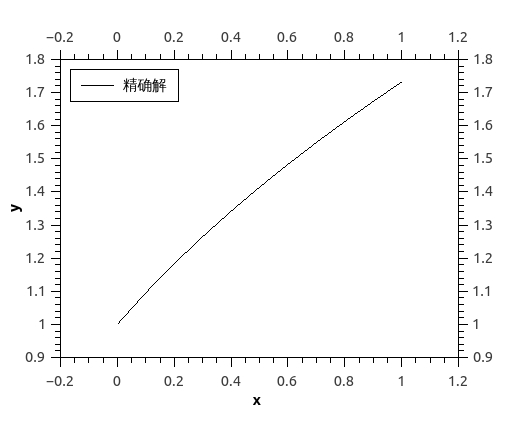
\includegraphics[width=0.9\textwidth]{program/numerical_analysis_examples/exact_solution.jpeg}
\caption{精确解}
\label{fig:by:table}
\end{minipage}
\end{figure}

Fortran代码如下:
\lstinputlisting{program/numerical_analysis_examples/exact_solution.f90}



\subsection{欧拉法求解}
对于解初值问题
$$\begin{cases}y\rq{}=y-\frac{2x}{y} &(0 \le x \le 1)\\ y(0)=1\end{cases}$$
的欧拉公式的具体形式为
$$y_{n+1}=y_n+h(y_n-\frac{2x_n}{y_n})$$
取步长为$h=0.1$其结果为

\begin{figure}[htb]
\begin{minipage}[b]{0.5\textwidth}
\centering
\begin{tabular}{c|c|c}
$x_n$ &       精确解($y_n$)   & 欧拉法解($y$)  \\
\hline
 0.0  &      1.000000       &	1.000000\\
 0.1	&	1.095445 	&	1.100000\\
0.2	&	1.183216 	&	1.191818\\
0.3	&	1.264911 	&	1.277438\\
0.4	&	1.341641	&	1.358213\\
0.5	&	1.414214	&	1.435133\\
0.6	&	1.483240	&	1.508966\\
0.7	&	1.549193	&	1.580338\\
0.8	&	1.612452	&	1.649784\\
0.9	&	1.673320	&	1.717780\\
1.0	&	1.732051	&	1.784771\\
\end{tabular}
\caption{精确解与欧拉法解}
\end{minipage}%
\begin{minipage}[b]{0.5\textwidth}
\centering
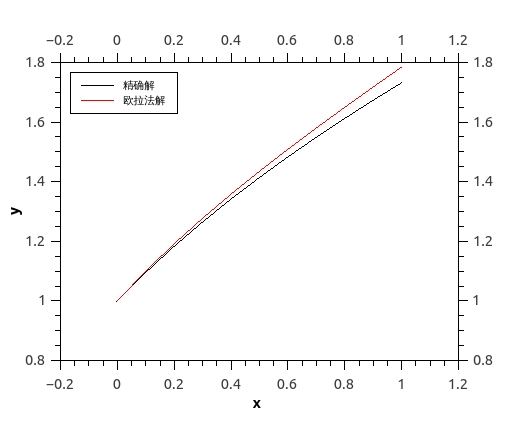
\includegraphics[width=0.9\textwidth]{program/numerical_analysis_examples/euler_method.jpeg}
\caption{精确解与欧拉法解}
\label{fig:by:table}
\end{minipage}
\end{figure}

Fortran代码如下:
\lstinputlisting[language=Fortran]{program/numerical_analysis_examples/euler_method.f90}



\subsection{改进欧拉法求解}
对于解初值问题
$$\begin{cases}y\rq{}=y-\frac{2x}{y} &(0 \le x \le 1)\\ y(0)=1\end{cases}$$
的改进欧拉公式的具体形式为
$$\begin{cases}
y_p=y_n+h(y_n-\frac{2x_n}{y_n})\\
y_c=y_n+h(y_p-\frac{2x_{n+1}}{y_p})\\
y_{n+1}=\frac{1}{2}(y_p+y_c)
\end{cases}$$
取步长$h=0.1$结果为

\begin{figure}[htb]
\centering
\begin{tabular}{c|c|c|c}
$x_n$ &       精确解($y_n$)   & 欧拉法解($y$)  & 改进欧拉法解($y$)\\
\hline
 0.0  &      1.000000       &	1.000000	&1.000000\\
 0.1	&	1.095445 	&	1.100000	&1.095909\\
0.2	&	1.183216 	&	1.191818	&1.184096\\
0.3	&	1.264911 	&	1.277438	&1.266201\\
0.4	&	1.341641	&	1.358213	&1.343360\\
0.5	&	1.414214	&	1.435133	&1.416402\\
0.6	&	1.483240	&	1.508966	&1.485955\\
0.7	&	1.549193	&	1.580338	&1.552514\\
0.8	&	1.612452	&	1.649784	&1.616474\\
0.9	&	1.673320	&	1.717780	&1.678166\\
1.0	&	1.732051	&	1.784771	&1.737867
\end{tabular}
\caption{精确解、欧拉法解、改进欧拉法解}
\centering
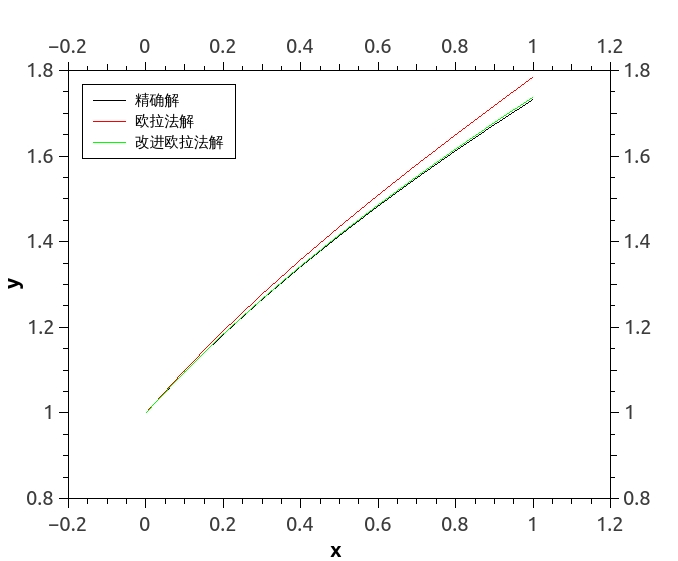
\includegraphics[width=0.7\textwidth]{program/numerical_analysis_examples/improved_euler_method.jpeg}
\caption{精确解、欧拉法解、改进欧拉法解}
\label{fig:by:table}
\end{figure}

Fortran代码如下:
\lstinputlisting[language=Fortran]{program/numerical_analysis_examples/improved_euler_method.f90}



\subsection{四阶龙格-库塔法求解}
对于解初值问题
$$\begin{cases}y\rq{}=y-\frac{2x}{y} &(0 \le x \le 1)\\ y(0)=1\end{cases}$$
的四阶龙格-库塔公式的具体形式为
$$\begin{cases}
y_{n+1}=y_n+\cfrac{h}{6}(K_1+2K_2+2K_3+K_4)\\
K_1=y_n-\cfrac{2x_n}{y_n}\\
K_2=y_n+\cfrac{h}{2}K_1-\cfrac{2x_n+h}{y_n+\cfrac{h}{2}K_1}\\
K_3=y_n+\cfrac{h}{2}K_2-\cfrac{2x_n+h}{y_n+\cfrac{h}{2}K_2}\\
K_4=y_n+hK_3-\cfrac{2(x_n+h)}{y_n+hK_3}
\end{cases}$$

Fortran代码如下:
\lstinputlisting[language=fortran]{program/numerical_analysis_examples/runge_kutta.f90}

取步长$h=0.1$结果为

\begin{figure}[htb]
\centering
\begin{tabular}{c|c|c|c|c}
$x_n$ &       精确解($y_n$)   & 欧拉法解($y$)  & 改进欧拉法解($y$) & 四阶龙格库塔法解($y$)\\
\hline
 0.0  &      1.000000       &	1.000000	&1.000000	&1.000000\\
 0.1	&	1.095445 	&	1.100000	&1.095909	&1.095446\\
0.2	&	1.183216 	&	1.191818	&1.184096	&1.183217\\
0.3	&	1.264911 	&	1.277438	&1.266201	&1.264912\\
0.4	&	1.341641	&	1.358213	&1.343360	&1.341642\\
0.5	&	1.414214	&	1.435133	&1.416402	&1.414215\\
0.6	&	1.483240	&	1.508966	&1.485955	&1.483242\\
0.7	&	1.549193	&	1.580338	&1.552514	&1.549196\\
0.8	&	1.612452	&	1.649784	&1.616474	&1.612455\\
0.9	&	1.673320	&	1.717780	&1.678166	&1.673324\\
1.0	&	1.732051	&	1.784771	&1.737867	&1.732056
\end{tabular}
\caption{精确解、欧拉法解、改进欧拉法解、四阶龙格库塔法解}
\centering
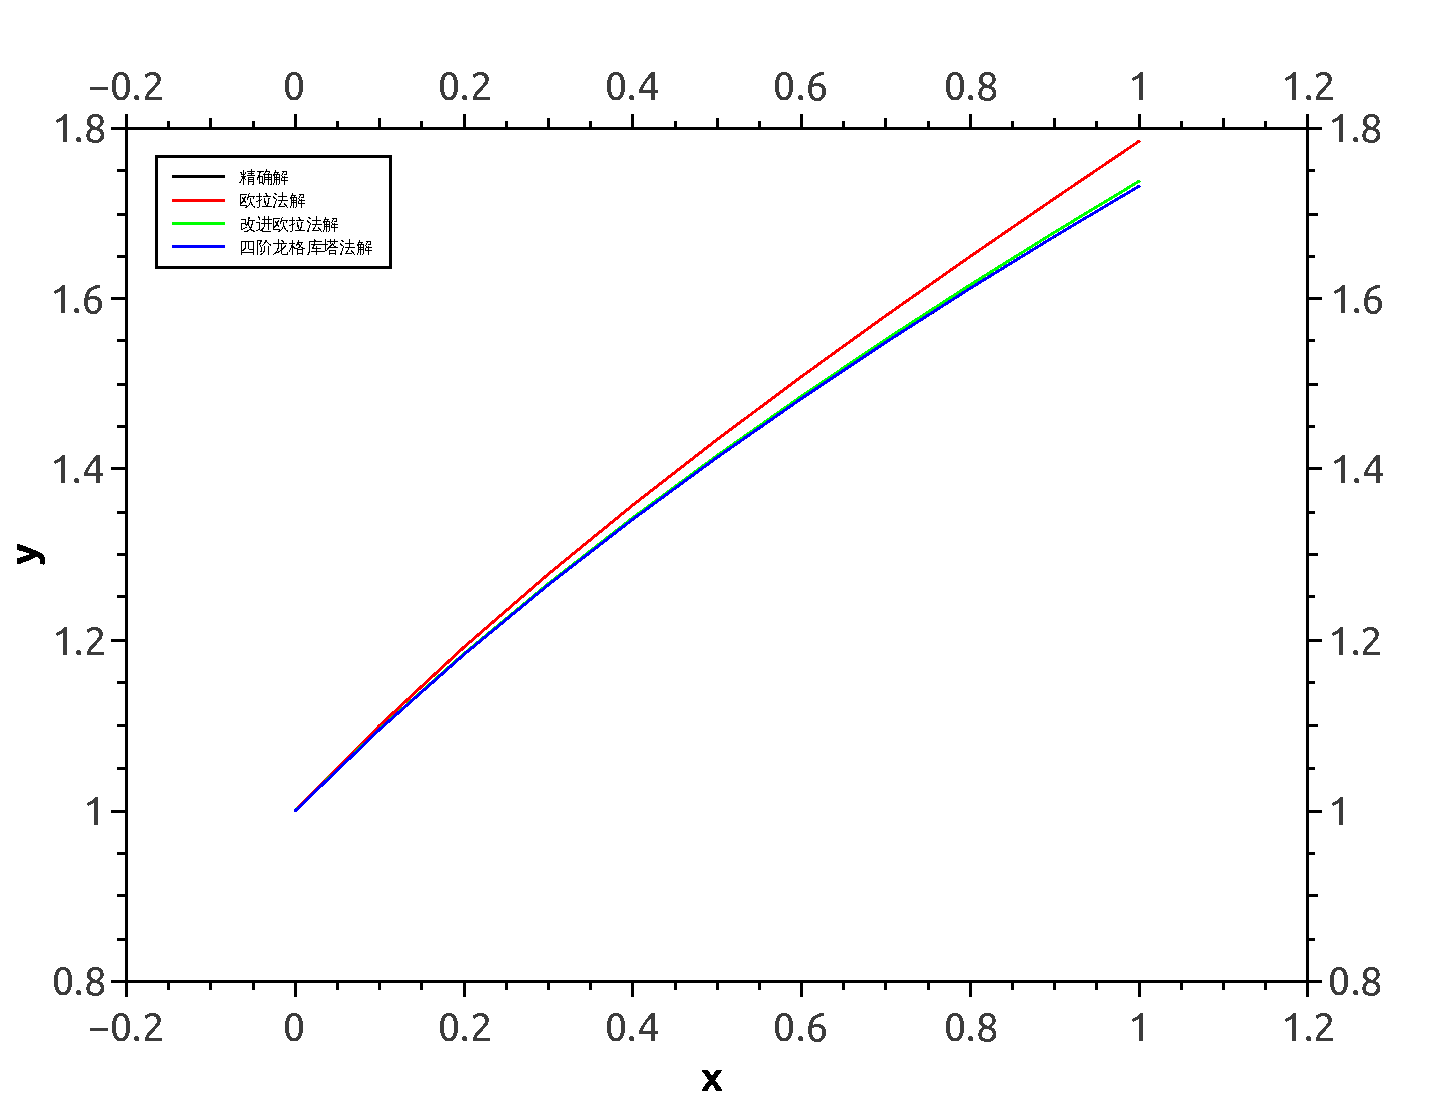
\includegraphics[width=1.0\textwidth]{program/numerical_analysis_examples/runge_kutta.pdf}
\caption{精确解、欧拉法解、改进欧拉法解、四阶龙格库塔法解}
\label{fig:by:table}
\end{figure}

四阶龙格库塔法的局部截断误差是$O(h^5)$,步长为$h=0.1$时,$h^5=0.00001$。

这个四阶龙格库塔的程序只适用于解这个问题,不具有普遍性,在四阶龙格库塔法程序章节中,将给出具有普遍性的四阶龙格库塔法的程序,而且适用于微分方程组。



\section{四阶龙格库塔法程序}

参考资料:《数值分析》(第4版),李庆扬,王能超,易大义 编;清华大学出版社


龙格-库塔法的推导基于泰勒展开,因而它要求所求的解具有较好的光滑性质。反之,如果解的光滑性差,那么实用四阶龙格-库塔法求得的数值解,其精度可以能反而不如改进的欧拉法。

一阶常微分方程的一般形式为:
$$\begin{cases}\cfrac{dy}{dx}=f(x,y),&a\le x\le b\\
y(a)=c &\end{cases}$$
在求解常微分方程时,通常会给出初始条件$x_0$及$y_0$。采用龙格库塔法求解常微分方程时,如果$x_1=x_0+h$,则对应的$y_1$为:
$$y_1=y_0+\frac{h}{6}(K_1+2\times K_2 +2\times K_3 + K_4)$$
其中4个参数为:
\begin{align*}
K_1&=f(x_0,y_0)\\
K_2&=f(x_0+\frac{h}{2},y_0+\frac{h}{2}K1)\\
K_3&=f(x_0+\frac{h}{2},y_0+\frac{h}{2}K2)\\
K_4&=f(x_0+h,y_0+hK_3)
\end{align*}

方程确定了,它的解也确定了\footnote{当然了,这个方程是有解的;还有就是有了初始条件或边界条件是唯一解,没这个是通解}。数值解是近似解,不同的步长有不同的精度,但是不管取何种步长,得出的解都是向精确解靠拢的。所以,当我们对同一个$x$值,用不同步长的到的$y$值相差很少时,说明这是时的解与精确解也相差很小,如果满足我们的精度需求,我们就可以取这时的$y$值。



\subsection{四阶龙格库塔法求解一阶微分方程组}

前面都是单个方程$y\rq{}=f$的数值解法,只要把$y$和$f$理解为向量,那么,所提供的各种计算公式即可应用到一阶方程组的情形。(还真没理解到?)

考察一阶方程组
$$y\rq{}_i=f_i(x,y_1,y_2,\cdots,y_N)\qquad (i=1,2,\cdots,N)$$
的初值问题,初始条件给为
$$y_i(x_0)=y_{i;0}\qquad (i=1,2,\cdots,N)$$
若采用向量的记号,记
$$\vec{y}=\begin{pmatrix}y_1 \\ y_2 \\ \vdots \\ y_N\end{pmatrix}
\qquad
\vec{y_0}=\begin{pmatrix} y_{1;0} \\ y_{2;0} \\  \vdots \\ y_{N;0} \end{pmatrix}
\qquad
\vec{f} =\begin{pmatrix} f_1 \\ f_2 \\ \vdots \\  f_N \end{pmatrix}$$
则上述方程组的初值问题可表示为
$$\begin{cases}\vec{y}\rq{}=\vec{f}(x,\vec{y}) \\ \vec{y}(x_0)=\vec{y}_0 \end{cases}$$
求解这一初值问题的四阶龙格-库塔公式为

(1)
$$\vec{y}_{n+1}=\vec{y}_n+\frac{h}{6}(\vec{k}_1+2\vec{k}_2+2\vec{k}_3+\vec{k}_4)$$
其中
$$\begin{cases}
\vec{k}_1 = \vec{f}(x_n,\vec{y}_n)\\
\vec{k}_2 = \vec{f}(x_n+\frac{h}{2},\vec{y}_n+\frac{h}{2}\vec{k}_1)\\
\vec{k}_3 = \vec{f}(x_n+\frac{h}{2},\vec{y}_n+\frac{h}{2}\vec{k}_2)\\
\vec{k}_4=\vec{f}(x_n+h,\vec{y}_n+h\vec{k}_3) 
 \end{cases}$$
或表示为

(2)
$$y_{i;n+1}=y_{i;n}+\frac{h}{6}(K_{i;1}+2K_{i;2}+2K_{i;3}+K_{i;4}) \qquad (i=1,2,\cdots,N)$$
其中
$$\begin{cases}
K_{i;1}=f_i(x_n,y_{1;n},y_{2;n},\cdots,y_{N;n})\\
K_{i;2}=f_i(x_n+\frac{h}{2},y_{1;n}+\frac{h}{2}K_{1;1},y_{2;n}+\frac{h}{2}K_{2;1},\cdots,y_{N;n}+\frac{h}{2}K_{N;1})\\
K_{i;3}=f_i(x_n+\frac{h}{2},y_{1;n}+\frac{h}{2}K_{1;2},y_{2;n}+\frac{h}{2}K_{2;2},\cdots,y_{N;n}+\frac{h}{2}K_{N;2})\\
K_{i;4}=f_i(x_n+h,y_{1;n}+hK_{1;3},y_{2;n}+hK_{2;3},\cdots,y_{N;n}+hK_{N;3})
\end{cases}
$$
{\color{red}本质上就是要包含,各个应变量,在hierachy中,$i$由$n,j_1,j_2,j_3$四个数来表征,可以考虑用四维数组表示!}

下标多了,容易搞混,一定要搞清楚。

$y_{i;n}$是第$i$个因变量$y_i(x)$在节点$x_n=x_0+nh$的近似值。分号“;”属于下标中,不要搞混。下标$i$(下标中的第一个数字)表征的是方程组中的方程序号,指的是具体的哪个方程,搞清到底有多少个方程是必要的!



\subsubsection{便于编程的形式}
为了方便编程,将方程组中的方程浓缩为一个一维数组来表示,长度就是方程组的个数。这意味着,矩阵运算将很方便。而且龙格库塔法作为一个子程序,循环利用,我们只需考虑第一步和第二步,始终是前一步是后一步的初值。
$$y_{1}(i)=y_{0}(i)+\frac{h}{6}\Big(K_{1}(i)+2K_{2}(i)+2K_{3}(i)+K_{4}(i)\Big) \qquad (i=1,2,\cdots,N)$$

可见$N$就是方程组中方程的个数。

其中
$$\begin{cases}
K_{1}(i)=f_i\big(x_0,y_{0}(1),y_{0}(2),\cdots,y_{0}(N)\big)\\
\qquad x_0\rq{}=x_0+\frac{h}{2} ,\quad y_{0}\rq{}(1)= y_{0}(1)+\cfrac{h}{2}K_{1}(1),
\quad   y_{0}\rq{}(2)=y_{0}(2)+\cfrac{h}{2}K_{1}(2), \cdots,y_{0}\rq{}(N)=y_{0}(N)+\frac{h}{2}K_{1}(N)\\
K_{2}(i)=f_i\big(x_0\rq{},y_{0}\rq{}(1),y_{0}\rq{}(2),\cdots,y_{0}\rq{}(N)\big)\\
\qquad x_0\rq{}\rq{}=x_0+\frac{h}{2} ,\quad y_{0}\rq{}\rq{}(1)= y_{0}(1)+\cfrac{h}{2}K_{2}(1),
\quad   y_{0}\rq{}\rq{}(2)=y_{0}(2)+\cfrac{h}{2}K_{2}(2),\cdots y_{0}\rq{}\rq{}(N)=y_{0}(N)+\frac{h}{2}K_{2}(N)\\
K_{3}(i)=f_i\big(x_0\rq{}\rq{},y_{0}\rq{}\rq{}(1),y_{0}\rq{}\rq{}(2),\cdots,y_{0}\rq{}\rq{}(N)\big)\\
\qquad x_0\rq{}\rq{}\rq{}=x_0+h ,\quad y_{0}\rq{}\rq{}\rq{}(1)= y_{0}(1)+hK_{3}(1),
\quad   y_{0}\rq{}\rq{}\rq{}(2)=y_{0}(2)+hK_{3}(2),\cdots, y_{0}\rq{}\rq{}\rq{}(N)=y_{0}(N)+hK_{3}(N)\\
K_{4}(i)=f_i\big(x_0\rq{}\rq{}\rq{},y_{0}\rq{}\rq{}\rq{}(1),y_{0}\rq{}\rq{}\rq{}(2),\cdots,y_{0}\rq{}\rq{}\rq{}(N)\big)\\
\end{cases}
$$
经过以上的变形,$K_1(i),K_2(i),K_3(i),K_4(i)$基本就有了个一致的造型,就是变量不同,而变量不同,另外赋值就可以了。可见代出初值进方程这个过程是可以重复利用的。知道注意的是,程序中,除了$f_i(\cdots)$是个函数外,$y$什么的都是数了。

\hypertarget{program}{\textbf{非数学语言表述就是:}}
\begin{enumerate}
\item 代入初值求得各个方程的值$f_i(\cdots)$,表示为$K_{1;i}$
\item 对变量进行处理,又作为初值代入各个方程中,求得其值$f_i(\cdots)$,只不过这次求的值表示为$k_{2;i}$。变量处理是,前次$x$值加半个步长$\frac{h}{2}$,即$x\rq{}_0=x_0+\frac{h}{2}$;而$y$是前次$y_i$加乘以半个步长$\frac{h}{2}$对应的$K_{1;i}$,即$y\rq{}_i=y_i+\frac{h}{2}K_{1;i}$
\item 又对变量进行处理,又作为初值代入各个方程中,求得其值$f_i(\cdots)$,这次求的值表示为$k_{3;i}$。这次变量处理与上次相似,只是$K_{1;i}$变成$K_{2;i}$。
\item 再次对变量进行处理,又作为初值代入各个方程中,求得其值$f_i(\cdots)$,这次求的值表示为$k_{4;i}$。这次变量处理与上两回稍有不同,乘的不是半步长,而是一个步长。
\end{enumerate}
上面的数学描述是针对一维数组的形式。但是只要实现非数学语言表述的求值过程,采用任何形式都是可以的。

具体的程序,参见举例。



\subsubsection{举例说明}
为了理解这一公式的计算过程,考察两个方程的特殊情形:
$$\begin{cases}
y_1\rq{}=f_1(x,y_1,y_2)\\
y_2\rq{}=f_2(x,y_1,y_2)\\
y_1(x_0)=y_{1;0}\\
y_2(x_0)=y_{2;0}
\end{cases}$$
四阶龙格-库塔公式的具体形式为
$$\begin{cases}
y_{1;n+1}=y_{1;n}+\frac{h}{6}(K_{1;1}+2K_{1;2}+2K_{1;3}+K_{1;4})\\
y_{2;n+1}=y_{2;n}+\frac{h}{6}(K_{2;1}+2K_{2;2}+2K_{2;3}+K_{2;4})\\
y_1(x_0)=y_{1;0}\\
y_2(x_0)=y_{2;0}
\end{cases}$$
其中
$$\begin{cases}
K_{1;1}=f_1(x_n,y_{1;n},y_{2;n})\\
K_{2;1}=f_2(x_n,y_{1;n},y_{2;n})\\
K_{1;2}=f_1(x_n+\frac{h}{2},y_{1;n}+\frac{h}{2}K_{1;1},y_{2;n}+\frac{h}{2}K_{2;1})\\
K_{2;2}=f_2(x_n+\frac{h}{2},y_{1;n}+\frac{h}{2}K_{1;1},y_{2;n}+\frac{h}{2}K_{2;1})\\
K_{1;3}=f_1(x_n+\frac{h}{2},y_{1;n}+\frac{h}{2}K_{1;2},y_{2;n}+\frac{h}{2}K_{2;2})\\
K_{2;3}=f_2(x_n+\frac{h}{2},y_{1;n}+\frac{h}{2}K_{1;2},y_{2;n}+\frac{h}{2}K_{2;2})\\
K_{1;4}=f_1(x_n+\frac{h}{2},y_{1;n}+\frac{h}{2}K_{1;3},y_{2;n}+hK_{2;3})\\
K_{2;4}=f_2(x_n+\frac{h}{2},y_{1;n}+\frac{h}{2}K_{1;3},y_{2;n}+hK_{2;3})
\end{cases}$$
编程的时候,不分第$n$个和$n+1$个,只有第0个和第1个值,其他循环套用就是了,即
$$\begin{cases}
y_{1;1}=y_{1;0}+\frac{h}{6}(K_{1;1}+2K_{1;2}+2K_{1;3}+K_{1;4})\\
y_{2;1}=y_{2;0}+\frac{h}{6}(K_{2;1}+2K_{2;2}+2K_{2;3}+K_{2;4})\\
y_1(x_0)=y_{1;0}\\
y_2(x_0)=y_{2;0}
\end{cases}$$
其中
$$\begin{cases}
K_{1;1}=f_1(x_0,y_{1;0},y_{2;0})\\
K_{2;1}=f_2(x_0,y_{1;0},y_{2;0})\\
K_{1;2}=f_1(x_0+\frac{h}{2},y_{1;0}+\frac{h}{2}K_{1;1},y_{2;0}+\frac{h}{2}K_{2;1})\\
K_{2;2}=f_2(x_0+\frac{h}{2},y_{1;0}+\frac{h}{2}K_{1;1},y_{2;0}+\frac{h}{2}K_{2;1})\\
K_{1;3}=f_1(x_0+\frac{h}{2},y_{1;0}+\frac{h}{2}K_{1;2},y_{2;0}+\frac{h}{2}K_{2;2})\\
K_{2;3}=f_2(x_0+\frac{h}{2},y_{1;0}+\frac{h}{2}K_{1;2},y_{2;0}+\frac{h}{2}K_{2;2})\\
K_{1;4}=f_1(x_0+\frac{h}{2},y_{1;0}+\frac{h}{2}K_{1;3},y_{2;0}+hK_{2;3})\\
K_{2;4}=f_2(x_0+\frac{h}{2},y_{1;0}+\frac{h}{2}K_{1;3},y_{2;0}+hK_{2;3})
\end{cases}$$



\subsection{定步长通用四阶龙格库塔程序}
为了有直观的理解,程序直接在举例中说明。对比这几个例子,可以发现,四阶龙格库塔法作为子程序subroutine rk4( xin , yin , n , h , yout) ,已经无需改动。对于不同的方程组,需要改动的仅是部分主体程序和全新的方程组子程序。
\subsubsection{一个微分方程求解举例}
仍然采用前面的例子:

求解初值问题
$$\begin{cases}y\rq{}=y-\frac{2x}{y} &(0 \le x \le 1)\\ y(0)=1\end{cases}$$

定步长通用四阶龙格库塔程序为

\lstinputlisting[language=Fortran]{program/runge_kutta/runge_kutta1.f90}
求解结果为:
{\small
\begin{center}
\begin{tabular}{c|c|c|c|c|c}
$x_n$  	&       精确解		  	& 四阶龙格库塔解		& 加强精度精确解	                 &通用四阶龙格库塔程序解	&	误差\\
\hline
 0.0  	&      1.000000       		&1.000000			&	1.00000000000000	&1.00000000000000		&	0\\
 0.1		&	1.095445 		&1.095446			&	1.09544511501033	&1.09544553169309		&	-4.16682760073783E-007\\
0.2		&	1.183216 		&1.183217			&	1.18321595661992	&1.18321674550599		&	-7.88886070024475E-007\\
0.3		&	1.264911 		&1.264912			&	1.26491106406735	&1.26491222834039		&	-1.16427303997746E-006\\
0.4		&	1.341641		&1.341642			&	1.34164078649987	&1.34164235375037		&	-1.56725050004525E-006\\
0.5		&	1.414214		&1.414215			&	1.41421356237310	&1.41421557789008		&	-2.0155169799807E-006\\
0.6		&	1.483240		&1.483242			&	1.48323969741913	&1.48324222277199		&	-2.52535285993893E-006\\
0.7		&	1.549193		&1.549196			&	1.54919333848297	&1.54919645230214		&	-3.11381917006415E-006\\
0.8		&	1.612452		&1.612455			&	1.61245154965971	&1.61245534965899		&	-0.0000038\\
0.9		&	1.673320		&1.673324			&	1.67332005306815	&1.67332465901626		&	-4.60594811002579E-006\\
1.0		&	1.732051		&1.732056			&	1.73205080756888	&1.73205636516556		&	-5.55759668019462E-006
\end{tabular}
\end{center}}
误差是“加强精度精确解”减“通用四阶龙格库塔程序解”所得的,看到冒出了很多小数位,那时因为最多显示14位小数所致。从误差可以看出,四阶龙格库塔法的解是相当精确的。步长是$0.1$,局部截断误差$0.1^5$=1.0E-004,实际误差比局部截断误差小很多。

\subsubsection{微分方程组求解举例}
用四阶龙格-库塔法求解常微分方程组
$$\begin{cases}
\cfrac{dy_0}{dx}=y_1\\
\cfrac{dy_1}{dx}=-y_0\\
\cfrac{dy_2}{dx}=-y_2\\
y_0(0)=-1,\quad y_1(0)=0,\quad y_2(0)=1
\end{cases}
\qquad 0\le x \le 1$$
这个问题的解析解是
$$y_0=-\cos x \qquad  y_1= \sin x  \qquad y_2 = e^{-x}$$

解析解的程序为

\lstinputlisting{program/runge_kutta/example3.f90}

定步长通用四阶龙格库塔程序为

\lstinputlisting{program/runge_kutta/runge_kutta3.f90}

定步长四阶龙格库塔法求解结果为

\begin{center}
\begin{tabular}{c|c|c|c}
	      $x_n$ 	&	    $ y_0$	       &         $y_1$	    &          $y_2$\\
	      \hline
          0.00000000        &-1.00000000         &0.00000000         &1.00000000\\
          0.05000000        &-0.99875026         &0.04997917         &0.95122943\\
          0.10000000        &-0.99500417         &0.09983341         &0.90483742\\
          0.15000000        &-0.98877108         &0.14943812         &0.86070798\\
          0.20000000        &-0.98006658         &0.19866932         &0.81873076\\
          0.25000000        &-0.96891242         &0.24740395         &0.77880079\\
          0.30000000        &-0.95533649         &0.29552019         &0.74081823\\
          0.35000000        &-0.93937272         &0.34289779         &0.70468810\\
          0.40000000        &-0.92106100         &0.38941832         &0.67032006\\
          0.45000000        &-0.90044711         &0.43496551         &0.63762817\\
          0.50000000        &-0.87758257         &0.47942552         &0.60653068\\
          0.55000000        &-0.85252454         &0.52268720         &0.57694983\\
          0.60000000        &-0.82533563         &0.56464245         &0.54881165\\
          0.65000000        &-0.79608382         &0.60518638         &0.52204580\\
          0.70000000        &-0.76484221         &0.64421766         &0.49658532\\
          0.75000000        &-0.73168889         &0.68163873         &0.47236657\\
          0.80000000        &-0.69670674         &0.71735606         &0.44932898\\
          0.85000000        &-0.65998318         &0.75128037         &0.42741495\\
          0.90000000        &-0.62161000         &0.78332688         &0.40656968\\
          0.95000000        &-0.58168313         &0.81341547         &0.38674104\\
          1.00000000        &-0.54030235         &0.84147095         &0.36787946\\
\end{tabular}
\end{center}

解析求解的结果及两种解误差为
{\small
\begin{center}
\begin{tabular}{c|c|c|c|c|c|c}
$x_n$	&	$y_0$解析解	&	$y_1$解析解	&	$y_2$解析解	&	$y_0$误差	&	$y_1$误差	&	$y_2$误差	\\
0.00	&	-1.00000000	&	0.00000000	&	1.00000000	&	0	&	0	&	0	\\
0.05	&	-0.99875026	&	0.04997917	&	0.95122942	&	0	&	0	&	0.00000001	\\
0.10	&	-0.99500417	&	0.09983342	&	0.90483742	&	0	&	-0.00000001	&	0	\\
0.15	&	-0.98877108	&	0.14943813	&	0.86070798	&	0	&	-0.00000001	&	0	\\
0.20	&	-0.98006658	&	0.19866933	&	0.81873075	&	0	&	-0.00000001	&	0.00000001	\\
0.25	&	-0.96891242	&	0.24740396	&	0.77880078	&	0	&	-0.00000001	&	0.00000001	\\
0.30	&	-0.95533649	&	0.29552021	&	0.74081822	&	0	&	-0.00000002	&	0.00000001	\\
0.35	&	-0.93937271	&	0.34289781	&	0.70468809	&	-0.00000001	&	-0.00000002	&	0.00000001	\\
0.40	&	-0.92106099	&	0.38941834	&	0.67032005	&	-0.00000001	&	-0.00000002	&	0.00000001	\\
0.45	&	-0.90044710	&	0.43496553	&	0.63762815	&	-0.00000001	&	-0.00000002	&	0.00000002	\\
0.50	&	-0.87758256	&	0.47942554	&	0.60653066	&	-0.00000001	&	-0.00000002	&	0.00000002	\\
0.55	&	-0.85252452	&	0.52268723	&	0.57694981	&	-0.00000002	&	-0.00000003	&	0.00000002	\\
0.60	&	-0.82533561	&	0.56464247	&	0.54881164	&	-0.00000002	&	-0.00000002	&	0.00000001	\\
0.65	&	-0.79608380	&	0.60518641	&	0.52204578	&	-0.00000002	&	-0.00000003	&	0.00000002	\\
0.70	&	-0.76484219	&	0.64421769	&	0.49658530	&	-0.00000002	&	-0.00000003	&	0.00000002	\\
0.75	&	-0.73168887	&	0.68163876	&	0.47236655	&	-0.00000002	&	-0.00000003	&	0.00000002	\\
0.80	&	-0.69670671	&	0.71735609	&	0.44932896	&	-0.00000003	&	-0.00000003	&	0.00000002	\\
0.85	&	-0.65998315	&	0.75128041	&	0.42741493	&	-0.00000003	&	-0.00000004	&	0.00000002	\\
0.90	&	-0.62160997	&	0.78332691	&	0.40656966	&	-0.00000003	&	-0.00000003	&	0.00000002	\\
0.95	&	-0.58168309	&	0.81341550	&	0.38674102	&	-0.00000004	&	-0.00000003	&	0.00000002	\\
1.00	&	-0.54030231	&	0.84147098	&	0.36787944	&	-0.00000004	&	-0.00000003	&	0.00000002	\\
\end{tabular}
\end{center}}

步长为$h=0.05$,局部截断误差为$h^5 =0.05^5=3.125\times 10^{-7}$



\subsection{自适应步长通用四阶龙格库塔程序}

\subsubsection{编程思想}

单从每一步看,步长越小,截断误差就越小,但随着步长的缩小,在一定求解范围内所要完成的步数就增加了。步数的增加不但引起计算量的增大,而且可能导致舍入误差的严重积累。因此微分方程的数值解法有个选择步长的问题。

在选择步长时,需要考虑两个问题:

1、怎样衡量和检验计算结果的精度?

2、如何依据所获得的精度处理步长?

以四阶龙格-库塔公式为例,从节点$x_n$出发,先以$h$为步长求出一个近似值,记为
$y_{h;n+1}$,由于公式的局部截断误差万恶诶$O(h^5)$,故有
$$y(x_{n+1}) - y_{h;n+1} \approx c h^5 $$
其中$y(x_{n+1})$是$x_{n+1}$处的精确解;$y_{h;n+1}$是$x_{n+1}$的数值近似解,$h$表示求解步长。

然后将步长折半,即取$\frac{h}{2}$为步长。从$x_n$跨两步到$x_{n+1}$,再求得一个近似值$y_{\frac{h}{2};n+1}$,每跨一步的截断误差是$c(\frac{h}{2})^2$,即
$$y(x_{n+1})-y_{h;n+1} \approx 2c\left(\frac{h}{2} \right)^5$$

比较上面两个截断误差公式,步长折半后,误差大约减少到$\frac{1}{16}$,即
$$\frac{y(x_{n+1})-y_{\frac{h}{2};n+1}}{y(x_{n+1})-y_{h;n+1}}\approx \frac{1}{16}$$
有
$$y(x_{n+1})-y_{\frac{h}{2};n+1}\approx \frac{1}{16}y(x_{n+1})-\frac{1}{16}y_{h;n+1}
\Longrightarrow
\frac{15}{16}y(x_{n+1}) \approx y_{\frac{h}{2};n+1} - \frac{1}{16}y_{h;n+1}
\Longrightarrow
y(x_{n+1}) \approx  \frac{16}{15}y_{\frac{h}{2};n+1}-\frac{1}{15}y_{h,n+1}$$
%
$$y(x_{n+1})-y_{\frac{h}{2};n+1}\approx \frac{1}{15}\left[ y_{\frac{h}{2};n+1}-y_{h,n+1}\right]$$

这样我们就可以通过折半前后两次计算结果的偏差
$$\Delta \equiv  y_{\frac{h}{2};n+1}-y_{h,n+1}$$
来判定所选的步长是否合适,具体地说,将区分以下两种情况处理:

1、对于给定的精度$\epsilon$,如果$\Delta > \epsilon$,我们反复将步长折半进行计算,直至$\Delta < \epsilon $为止,这时取最终得到的$y_{\frac{h}{2},n+1}$\footnote{这是经过$n$折半后的步长计算值,此时真实步长是$(\frac{h}{2})^n$}作为结果;

2、如果$\Delta < \epsilon$,我们将反复将步长加倍,直到$\Delta > \epsilon$为止,这时再将步长折半一次,就得到所要的结果。

显然通常情况下,我们只需考虑第一种情况就可以了,因为总要进行一次折半步长运算,所以变步长龙格库塔法步长可以选则比定步长龙格库塔法大些,大两倍。因为真实用到的步长是预先定义步长$h$的一半$\frac{h}{2}$。也无需考虑第二种情况,第一次步长折半算到的值就满足精度的话,就通过,直接算下一步。这里的两种情况是为了选择最佳步长,而我们的目的不是选则最佳步长,而是求得满足精度的值,所以无需考虑第二种情况。






\chapter{堆排序}
\url{http://blog.csdn.net/morewindows/article/details/6709644/}
\url{http://www.cnblogs.com/mengdd/archive/2012/11/30/2796845.html}
\url{http://www.cnblogs.com/jingmoxukong/p/4303826.html}

堆排序(Heap Sort),是一种选择排序,其时间复杂度为$O(n\log n)$。

堆排序方法对记录数较少的文件并不值得提倡,但对$n$较大的文件还是很有效的。因为其运行时间主要耗费在建初始堆和调整建新堆时进行的反复“筛选”上。

堆排序在最坏的情况下,其时间复杂度也为$O(n\log n)$。相对于快速排序来说,这是堆排序的最大优点。此外,堆排序仅需一个记录大小的供交换用的辅助存储空间。


\section{堆的定义}
数据结构中的二叉堆,是完全二叉树或者是近似完全二叉树。满足的特性为:
\begin{itemize}
\item 父结点的键值总是大于或等于(小于或等于)任何一个子节点的键值;
\item 每个结点的左子树和右子树都是一个二叉堆.
\end{itemize}
当父结点的键值总是大于或等于任何一个子节点的键值时为最大堆。当父结点的键值总是小于或等于任何一个子节点的键值时为最小堆。下图展示一个最小堆:

\begin{figure}[h]
\begin{center}
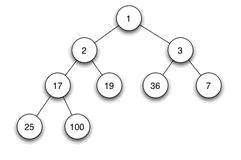
\includegraphics[width=0.4\textwidth]{pictures/heap.png}
\end{center}
\caption{小顶堆}
%\label{fig:las298}
\end{figure}

由于其它几种堆(二项式堆,斐波纳契堆等)用的较少,一般将二叉堆就简称为堆。



\section{堆的储存}
一般用数组来表示堆。

(1)以下标为“0”开始的$n$个元素的序列$\{k_0,k_1,\cdots, k_{n-1}\}$当且仅当满足下列关系时
\begin{itemize}
\item 情形1:$\begin{cases}
k_i \le k_{2i+1}\\
k_i \le k_{2i+2}
\end{cases}$,称之为最小化堆或小顶堆;
\item 情形2:$\begin{cases}
k_i \ge k_{2i}\\
k_i \ge k_{2i+1}
\end{cases}$,称之为最大化堆或大顶堆。
\end{itemize}
其中$i=0,1,2,\cdots,(n/2-1)$向下取整。


(2)以下标为“1”开始的$n$个元素的序列$\{k_1,k_2,\cdots, k_n\}$当且仅当满足下列关系时
\begin{itemize}
\item 情形1:$\begin{cases}
k_i \le k_{2i}\\
k_i \le k_{2i+1}
\end{cases}$,称之为最小化堆或小顶堆;
\item 情形2:$\begin{cases}
k_i \ge k_{2i}\\
k_i \ge k_{2i+1}
\end{cases}$,称之为最大化堆或大顶堆。
\end{itemize}
其中$i=1,2,\cdots,n/2$向下取整。


\section{堆排序的思想}
有了堆的定义,就自然过渡到堆排序了。一个无序数组,如果构造成了大顶堆,这就筛选出了这个数组的最大值,即第一项(堆顶值)。此时,我们把这个最大值取出,余下的部分继续构造成大顶堆,继续取出堆顶值,反复进行就实现了原来数组的排序。但是具体操作可以变得更为有效:排序开始,首先输出堆顶元素(因为它是最值),将堆顶元素和最后一个元素交换,这样,第$n$个位置(即最后一个位置)作为有序区,前$n-1$个位置仍是无序区,对无序区进行调整,得到堆之后,再交换堆顶和最后一个元素,这样有序区长度变为$2\cdots$不断进行此操作,将剩下的元素重新调整为堆,然后输出堆顶元素到有序区。每次交换都导致无序区$-1$,有序区$+1$。不断重复此过程直到有序区长度增长为$n-1$,排序完成。由排序过程可见,若想得到升序,则建立大顶堆,若想得到降序,则建立小顶堆。

在将堆顶元素和最后一个元素交换后形成的无序区重新构建堆也是有规律可循的。这也是堆调整的最关键部分。每个子树根都是该子树分支的最值。当堆的根元素与最后一个元素交换后,重新构建堆,实际就是将处于根位置的新元素不断与子结点比较,下沉到树中的合适位置。每次完成比较,另一支子树就不用考虑,减少$1/2$需要比较的数据量。这是堆的特性所决定的,因为每个父节点都是所处树分枝的最值,无论这个树分枝是大还是小。这是堆调整的核心要点。后面会有具体例子说明。



以上思想可归纳为两个操作:
\begin{enumerate}[(1)]
\item 根据初始数组去构造初始堆(以大顶堆为例,构建一个完全二叉树,保证所有的父结点都比它的孩子结点数值大)。初始化堆的时候是对所有的非叶子结点进行筛选。最后一个非终端元素的下标是$n/2$向下取整,所以筛选只需要从第$n/2$向下取整个元素开始,从后往前进行调整。每次都是从父结点、左孩子、右孩子中进行比较交换,交换可能会引起孩子结点不满足堆的性质,所以每次交换之后需要重新对被交换的孩子结点进行调整。
\item 每次交换第一个和最后一个元素,输出最后一个元素(最大值),然后把剩下元素重新调整为大根堆。
其中调整建堆的方法是,将根结点值与左、右子树的根结点值进行比较,若不满足堆的条件,则将左、右子树根结点值中的大者与根结点值进行交换。未被破坏的子树就不用管了,然后顺着被破坏的子树一路调整下去,直至叶子结点,就得到新的堆。(牢牢记住堆的特性,父结点是所处子树的最值。堆中有相同元素也没关系,堆的定义特性在于保证堆顶是最值。即堆只能保证堆中元素的最值。对于排序,有这点就够了。)
\end{enumerate}
当输出完最后一个元素后,这个数组已经是按照从小到大的顺序排列了。



\newpage
\section{堆排序实例}
(1)以构建大顶堆实现从小到大排序为例。建立初始的堆结构如图
\begin{figure}[h]
\begin{center}
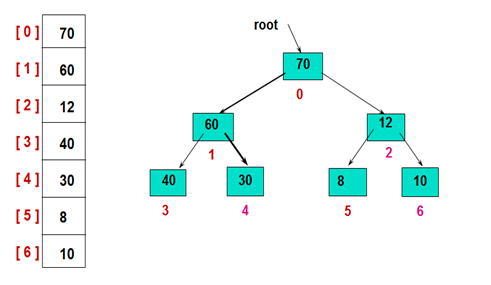
\includegraphics[width=0.5\textwidth]{pictures/2012113021435914.png}
\end{center}
%\caption{小顶堆}
%\label{fig:las298}
\end{figure}

(2)然后,交换堆顶的元素和最后一个元素,此时最后一个位置作为有序区(有序区显示为黄色)
\begin{figure}[h]
\begin{center}
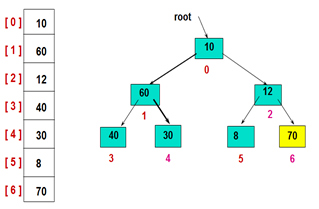
\includegraphics[width=0.5\textwidth]{pictures/heapsort1.png}
\end{center}
%\caption{小顶堆}
%\label{fig:las298}
\end{figure}

(3)每个子树根都是该子树分支的最大值。而子树根60比子树根12大,12 所在的子树无需考虑,此时一半的数据量无需比较。10比60小,60是整个序列的第二大值。交换10和60,此时筛选出了第二大值。但是为了保证余下的排序,仍要继续调整10至合适位置,直至重新构建成一个堆。
\begin{figure}[h]
\begin{center}
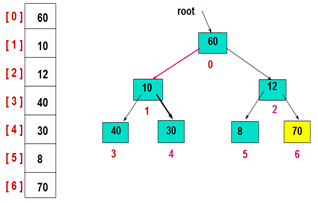
\includegraphics[width=0.5\textwidth]{pictures/heapsort2.png}
\end{center}
%\caption{小顶堆}
%\label{fig:las298}
\end{figure}

\newpage
(4)10不断下沉至合适位置,每次调整,减少余下的一半的数据去比较。此时蓝色部分重新构建称为堆。
\begin{figure}[h]
\begin{center}
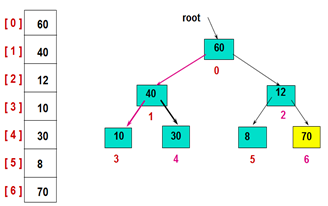
\includegraphics[width=0.5\textwidth]{pictures/heapsort3.png}
\end{center}
%\caption{小顶堆}
%\label{fig:las298}
\end{figure}

(5)进入第二轮排序,60与堆中最后一个元素交换位置。
\begin{figure}[h]
\begin{center}
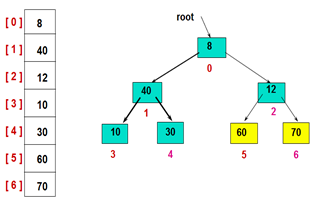
\includegraphics[width=0.5\textwidth]{pictures/heapsort4.png}
\end{center}
%\caption{小顶堆}
%\label{fig:las298}
\end{figure}


(6)又开始调整堆。
\begin{figure}[h]
\begin{center}
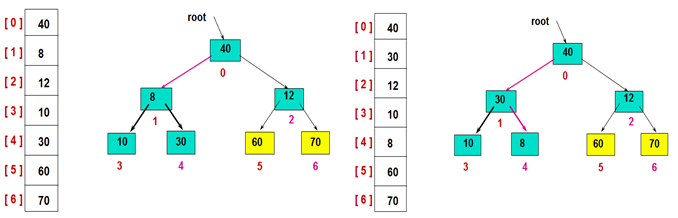
\includegraphics[width=0.9\textwidth]{pictures/heapsort5.png}
\end{center}
%\caption{小顶堆}
%\label{fig:las298}
\end{figure}

\newpage
(7)重复此过程。
\begin{figure}[h]
\begin{center}
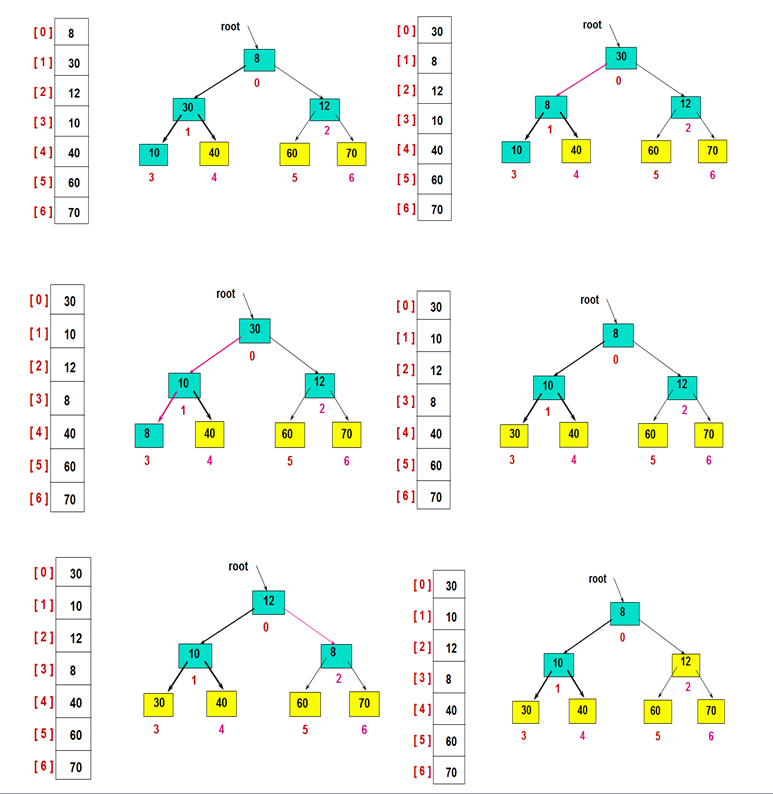
\includegraphics[width=0.75\textwidth]{pictures/2012113021474819.png}
\end{center}
%\caption{小顶堆}
%\label{fig:las298}
\end{figure}

(8)最后,有序区扩展完成即排序完成。
\begin{figure}[h]
\begin{center}
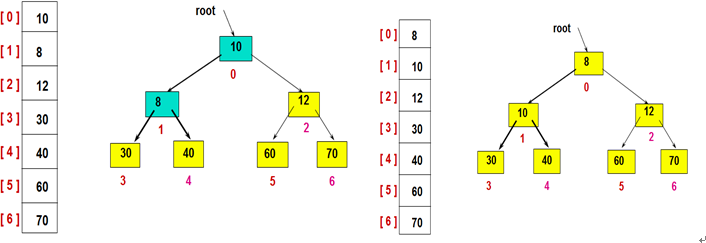
\includegraphics[width=0.75\textwidth]{pictures/2012113021482583.png}
\end{center}
%\caption{小顶堆}
%\label{fig:las298}
\end{figure}




\chapter{差分进化算法}
\section{背景}
\url{https://www.cnblogs.com/tsingke/p/5809453.html}

DE算法-作者网站: \url{http://www1.icsi.berkeley.edu/~storn/code.html}

维基百科资料库  : \url{https://en.wikipedia.org/wiki/Differential_evolution}

差分进化算法(Differential Evolution,DE)是由Storn等人于1995年提出的,和其它演化算法一样,DE是一种模拟生物进化的随机模型,通过反复迭代,使得那些适应环境的个体被保存了下来。但相比于进化算法,DE保留了基于种群的全局搜索策略,采用实数编码、基于差分的简单变异操作和一对一的竞争生存策略,降低了遗传操作的复杂性。同时,DE特有的记忆能力使其可以动态跟踪当前的搜索情况,以调整其搜索策略,具有较强的全局收敛能力和鲁棒性,且不需要借助问题的特征信息,适于求解一些利用常规的数学规划方法所无法求解的复杂环境中的优化问题。目前,DE已经在许多领域得到了应用,譬如人工神经元网络、化工、电力、机械设计、机器人、信号处理、生物信息、经济学、现代农业、食品安全、环境保护和运筹学等。
 
 
DE 算法主要用于求解连续变量的全局优化问题,其主要工作步骤与其他进化算法基本一致,主要包括变异(Mutation)、交叉(Crossover)、选择(Selection)三种操作。算法的基本思想是从某一随机产生的初始群体开始,利用从种群中随机选取的两个个体的差向量作为第三个个体的随机变化源,将差向量加权后按照一定的规则与第三个个体求和而产生变异个体,该操作称为变异。然后,变异个体与某个预先决定的目标个体进行参数混合,生成试验个体,这一过程称之为交叉。如果试验个体的适应度值优于目标个体的适应度值,则在下一代中试验个体取代目标个体,否则目标个体仍保存下来,该操作称为选择。在每一代的进化过程中,每一个体矢量作为目标个体一次,算法通过不断地迭代计算,保留优良个体,淘汰劣质个体,引导搜索过程向全局最优解逼近。


\section{具体步骤}
{\small\url{https://pablormier.github.io/2017/09/05/a-tutorial-on-differential-evolution-with-python/}}

\url{https://blog.csdn.net/qq_37423198/article/details/77856744}

\paragraph{目的} 对于一个黑箱函数,有一组参数,设参数个数为$N$。利用差分进化算法来寻找黑箱函数最小值的参数。
\begin{equation}
f(x_1,x_2,x_3,\cdots,x_N)
\end{equation}

\paragraph{定义} 将黑箱函数的一组参数称为个体;多组参数(个体)称为种群。
 
\paragraph{第〇步} 初始化种群(产生初始值):产生大小为$M$的种群,即包含$M$组参数($M$个个体)。$M$的选择一般介于参数个数$N$的5到10倍之间

\begin{itemize}
\item 设定每个参数的取值边界范围。
\begin{equation}
(b_{j-min},b_{j-max}),\quad j = 1, 2, 3, \cdots, N
\end{equation}
\item 随机产生$M$个个体($M$组参数);也可以加入自己设定的初始值。
\begin{align}
X_i(0) &= \{x_{i,1}(0),x_{i,2}(0),x_{i,3}(0),\cdots, x_{i,N}(0)\}\\
&=\begin{pmatrix}
x_{1,1}(0) & x_{1,2}(0) &x_{1,3}(0) &\cdots &x_{1,N}(0)\\
x_{2,1}(0) & x_{2,2}(0) &x_{2,3}(0) &\cdots &x_{2,N}(0)\\
x_{3,1}(0) & x_{3,2}(0) &x_{3,3}(0) &\cdots &x_{1,N}(0)\\
\vdots      &   \vdots     & \vdots      & \cdots & \vdots \\
x_{M,1}(0) & x_{M,2}(0) &x_{M,3}(0) &\cdots &x_{M,N}(0)
\end{pmatrix}
\end{align}
其中
\begin{align}
x_{i,j}(0) &= b_{j-min} + rand(0,1)* (b_{j-max}-b_{j-min})\\
 i &= 1,2,3,\cdots, M\\
 j &= 1,2,3,\cdots, N
\end{align}
\item 代入到黑箱函数计算,得出最优值。
\end{itemize}


\paragraph{第一步} 变异(按照特定策略修改参数):对之前产生的$M$个个体逐个进行变异。
\begin{itemize}
\item 变异方法:对$i$个个体进行变异,则再随机选择除第$i$个个体外的3个个体,表示为$a$、$b$、$c$,以特定的变异策略计算变异体。存在多种变异策略,以最简单的“rand1bin”为例
\begin{equation}
x_{i-mut} = a + mut * (b-c)
\end{equation}
其中$mut$是变异因子(缩放因子),取值一般在$[0.5,2]$之间。 大的变异因子可以扩大搜索范围,但是会降低收敛速度。
\item 变异策略:
\begin{itemize}
\item Rand/1: $x_{mut} = x_{r1} + mut*(x_{r2}-x_{r3})$
\item Rand/2: $x_{mut} =x_{r1} + mut*(x_{r2}-x_{r3}+x_{r4}-x_{r5})$
\item Best/1: $x_{mut}=x_{best}+mut*(x_{r2}-x_{r3})$
\item Rand-to-best/1: $x_{mut}=x_{r1}+mut_1 *(x_{r2}-x_{r3}) + mut_2*(x_{best}-x_{r1})$
\item $\cdots$
\end{itemize}
\item 自适应变异因子:暂略!
\end{itemize}



\paragraph{第二步} 交叉(将修改后的参数和原参数按照特定策略进行取舍,得到新参数):将变异体和未变异体进行混合,即将两者参数进行混合。
\begin{itemize}
\item 交叉策略:对应于每个参数,产一个随机数,将这个随机数与设定交叉因子做对比。如果小于这个因子,就保留变异体中的这个参数,否在就保留原参数。这样就实现了变异体和未变异体的混合。
\begin{equation}
x_{i,j}^{new} =\begin{cases}
x_{i,j}^{mut},& rand(0,1)\le cr\\
x_{i,j}^{ori}, &else
\end{cases}
\end{equation}

其中$cr \in [0,1]$为交叉概率。这个策略称为二项式交叉策略(Binomial crossover, bin)。还有在两组参数中随机挑选参数的指数交叉策略(Exponential crossover, exp)。

\item 自适应交叉因子:暂略!
\end{itemize}

\paragraph{第三步} 选择(对比新参数和原参数的函数值,保留最优值)


至此得到一个全新的种群。将这个全新的种群重复后三个步骤(变异、交叉、选择),进行迭代,直至找到最优解。





\chapter{数值计算库}
\section{Intel MKL}
\subsection{Intel MKL简介}
Intel数学核心函数库(Math Kernel Library, MKL)是一套高度优化、线程安全的数学例程、函数,面向高性能的工程、科学与财务应用。英特尔 MKL 的集群版本包括 ScaLAPACK 与分布式内存快速傅立叶转换,并提供了线性代数 (BLAS、LAPACK 和Sparse Solver)、快速傅立叶转换、矢量数学 (Vector Math) 与随机号码生成器支持。

主要包括:

① LAPACK (线形代数工具linear algebra package)

② DFTs (离散傅立叶变换 Discrete Fourier transforms)

③ VML (矢量数学库Vector Math Library)

④ VSL (矢量统计库Vector Statistical Library)

 
MKL的主要功能:

1)BLAS 和 LAPACK

在英特尔处理器中部署经过高度优化的基本线性代数例程BLAS(Basic Linear Algebra Subroutines)和 线性代数包LAPACK(Linear Algebra Package) 例程,它们提供的性能改善十分显著。
 
2)ScaLAPACK

ScaLAPACK是一个并行计算软件包,适用于分布存储的MIMD并行机。ScaLAPACK提供若干线性代数求解功能,具有高效、可移植、可伸缩、高可靠性的特点,利用它的求解库可以开发出基于线性代数运算的并行应用程序。
ScaLAPACK 的英特尔? MKL 实施可提供显著的性能改进,远远超出标准 NETLIB 实施所能达到的程度。
 
3)PARDISO稀疏矩阵解算器

利用 PARDISO 直接稀疏矩阵解算器解算大型的稀疏线性方程组,该解算器获得了巴塞尔大学的授权,是一款易于使用、具备线程安全性、高性能的内存高效型软件库。英特尔? MKL 还包含共轭梯度解算器和 FGMRES 迭代稀疏矩阵解算器。
 
4)快速傅立叶变换 (FFT)

充分利用带有易于使用的新型 C/Fortran 接口的多维 FFT 子程序(从 1 维至 7 维)。英特尔? MKL 支持采用相同 API 的分布式内存集群,支持将工作负载轻松地分布到大量处理器上,从而实现大幅的性能提升。此外,英特尔? MKL 还提供了一系列 C 语言例程(“wrapper”),这些例程可模拟 FFTW 2.x 和 3.0 接口,从而支持当前的 FFTW 用户将英特尔? MKL 集成到现有应用中。
 
5)矢量数学库(VML)

矢量数学库(Vector Math Library)借助计算密集型核心数学函数(幂函数、三角函数、指数函数、双曲函数、对数函数等)的矢量实施显著提升应用速度。
 
6)矢量统计库—随机数生成器(VSL)

利用矢量统计库(Vector Statistical Library)随机数生成器加速模拟,从而实现远远高于标量随机数生成器的系统性能提升。


\subsection{命名规则}
【注】这里只是简单的介绍,一切以MKL的技术手册为准,在技术手册的头几个章节就有说明。技术手册网上有,MKL安装后也有份本地文件。这个在下面的使用心得中有详细介绍。

Naming Conventions

Argument types. Types of all arguments of Fortran routines in this Quick Reference follow these conventions:
\begin{itemize}
\item IMPLICIT COMPLEX (C) 
\item IMPLICIT DOUBLE PRECISION (D) 
\item IMPLICIT INTEGER (I-N) 
\item IMPLICIT DOUBLE COMPLEX (Z) 
\item CHARACTER*1 compq, compz, diag, eigsrc, howmny, initv, job, norm, order, range, side, trans, transa, transb, uplo, vect 
LOGICAL select
\end{itemize}

Arrays. Names of Fortran arrays are typeset in UPPERCASE letters, and names of all other Fortran arguments are in lowercase letters. Code examples and data types for C interface are also given in lowercase.

Names of routines. The first letter of a routine name identifies the type of the result: 
\begin{itemize}
\item s    SINGLE 
\item d    DOUBLE PRECISION 
\item c    COMPLEX 
\item z    DOUBLE COMPLEX 
\item i    INTEGER
\end{itemize}

Function names for C interface are given in lowercase courier mixed with UpperCase courier.

To specify the group of routine names that differ in the first letter, this Quick Reference uses the question mark (?). For example, ?getrf refers to the routines sgetrf, dgetrf, cgetrf, and zgetrf.


\subsection{使用心得}
MKL用起来真的是不容易的,曲曲折折,当然了,这跟自己的Linux基础知识不够扎实有关。MKL是优化了很多现有的优秀的数学函数库。我本来想在C++直接调用这些库。后来觉得里面的BLAS原生就是用的Fortran写的,自己对Fortran熟悉,C++还不熟。所以还是一个台阶一个台阶的来吧,不然就函数接口而言估计都够折腾的,事实上Fortran 95的函数接口都折腾我够呛的。因为BLAS最初是Fortran 77写的。

先说下心得中最核心的一条:纵使你在网上搜到各种说法,万变不离其综的王道是,看MKL自带的技术手册,千多页呢,讲的不能再详细了。技术手册网上有,

\url{http://software.intel.com/sites/products/documentation/doclib/mkl_sa/11/mklman/index.htm}

安装后,本地文件也有。建议看本地文件的技术手册,与安装的版本对应,更全面,更直观。本地的技术手册,在安装目录下,Document 目录下找,所有的文档都在那。

第一天,云里雾里,什么都不知道。第二天,学会了看技术手册,是网页版的,从mkl\_documentation.htm开始。知道了命名规则,及各项参数,成功的用Fortran 77 函数接口调用了矩阵相乘的子程序。编译的时候很简单,多加个 -mkl 选项就可以了。以我的测试文件为例:\verb|ifort test1_ver1.f90 -mkl|

测试文件如下:
\lstinputlisting{program/test/test1_ver1.f90}

Fortran 95的函数接口简单,参量少,用起来方便,可是调用时屡屡出错:
\begin{verbatim}
In function `MAIN__':
test_ver2.f90:(.text+0x164): undefined reference to `dgemm_mkl95_'
\end{verbatim}

究其原因,应该是没有链接到合适的库。在mkl\_documentation.htm旁边有个
mkl\_link\_line\_advisor.htm文件,这个文件很有用。它能指出合适的链接和编译选项,只是生成链接和编译选项时,需要手动选择系统相关参数。如果系统相关参数不清楚,怎么办呢? 在 MKL的安装目录下,例如我的安装目录\verb|/opt/intel/mkl| 下有个tools目录,里面有个很有用的工具 mkl\_link\_tool。 直接运行这个程序就能得到这个程序的相关说明。如果加上参数 -check\_mkl\_presence运行,即 \verb|./mkl_link_tool -check_mkl_presence| 就能到自己安装的详细参数。用这些参数在mkl\_link\_line\_advisor.htm文件选择合适的选项,就能得到链接和编译选项,如我的:
\begin{verbatim}
Use this link line: 
$(MKLROOT)/lib/intel64/libmkl_blas95_lp64 
-L$(MKLROOT)/lib/intel64 
-lmkl_intel_lp64 -lmkl_core -lmkl_sequential -lpthread -lm

Compiler options: 
 -I$(MKLROOT)/include/intel64/lp64 -I$(MKLROOT)/include
\end{verbatim}
这里的链接和选项需要适当的调整,因为它不知道MKL的安装路径,这个要自己补充。要将\verb|$(MKLROOT)|替换成安装路径,我的安装路径为\verb|/opt/intel/mkl|。还有就是库文件libmkl\_blas95\_lp64是有后缀的,加上libmkl\_blas95\_lp64.a。这些库文件,自己可以在相应目录下看看。编译链接及编译选项都得加进去,于是最终有效的编译是:
\begin{verbatim}
ifort test1_ver2.f90 
/opt/intel/mkl/lib/intel64/libmkl_blas95_lp64.a 
-L/opt/intel/mkl/lib/intel64 
-lmkl_intel_lp64 -lmkl_core -lmkl_sequential -lpthread -lm 
-I/opt/intel/mkl/include/intel64/lp64 -I/opt/intel/mkl/include
\end{verbatim}
很长很麻烦,显然不是最终解决方案。

测试文件如下:
\lstinputlisting{program/test/test1_ver2.f90}






\section{FFTW}
\subsection{FFTW的简介}
官方网站:\url{http://www.fftw.org/}

下载地址:\url{http://www.fftw.org/download.html}

快速傅立叶变换(FFTW)是由麻省理工学院开发的免费的软件包,采用 C 语言编写,计算一维和多维离散傅立叶变换。FFTW 的编码生成器采用面向对象设计技术和面向对象语言Caml 编写;它能自动适应系统硬件,因而可移植性很强。FFTW2.1.5 支持共享存储多线程并行和分布式存储 MPI 并行。FFTW 的运算性能远远领先于目前已有的其它 FFT 软件。FFTW 为任意大小的模式生成一个计划(plan),通过对该计划施行各种运算完成各种模式的转换;内部结构及其复杂性对用户透明;速度快 (适合各种机器的内部编译器、代码生成器利用 AST 在运行时生成代码并自我优化,而且不占用编译时间,
采用分层存储技术)。FFTW 受到越来越多的科学研究和工程计算工作者的普遍青睐,并为量子物理、光谱分析、音视频流信号处理、石油勘探、地震预报、天气预报、概率论、编码理论、医学断层诊
断等领域提供切实可行的大规模 FFT 计算。


\subsection{安装调用}
(1)安装
\begin{itemize}
\item 切换到解压目录
\item 使用管理员权限 或在命令前直接加 sudo
\item ./configure
\item make
\item make check
\item make install
\end{itemize}

(2)调用

\verb*|ifort xx.f90 -lfftw3 -lm|


\subsection{实例}
在linux下有如下程序:
\begin{lstlisting}[language=Fortran]
program aab
	use fftw3
	implicit none 
	integer i , j , n
	parameter (n=8)
	type(C_PTR) :: plan
	complex(C_DOUBLE_COMPLEX), dimension(n,n) :: in, out
	do i=1,n
		do j=1,n
			in(i,j)=cmplx(cos(i*0.22),sin(j*0.3))
		enddo
	enddo
	out=0.d0
	plan =fftw_plan_dft_2d(n,n,in,out,FFTW_FORWARD,FFTW_ESTIMATE)
	call fftw_execute_dft(plan, in, out)
	write(777,*) real(out)
	write(777,*) aimag(out)
	call fftw_destroy_plan(plan)
	stop
end
\end{lstlisting}

编译 :gfotran -o x   x.f90 -lfftw3

运行:./x


\section{BLAS}
\subsection{BLAS简介}
官网:\url{http://www.netlib.org/blas/}

BLAS系Basic Linear Algebra Subprograms的缩写。顾名思义,BLAS实现基本的线性代数运算,是NetLib中一些高级软件包--比如,LAPACK和LINPACK-- 的“基石”。据说,BLAS由美国NSF和DOE资助,在1970s开始推出,至今仍在发展。这是一个PublicDomain的著名软件包。
     BLAS的基本部分由三个级别构成:第一级完成“向量-向量”操作;第二级实现“矩阵-向量”运算;第三级包含“矩阵-矩阵”程序。所有的子程序都经过精 心的优化以确保其高效性;程序的书写和语句的选择都相当规范,以便于移植。针对不同的平台,有多种经过低级别优化(比如汇编级优化)的BLAS库可供直接 使用。
     长期以来,专家们一直呼吁使用BLAS来建立和开发自己的线性代数软件包。这样做,不仅可以缩短开发周期,而且便于形成统一的调用接口。当BLAS升级 时,您可以坐享其成。由于源码是公开的,您不必担心受制于人(如果您使用商品化的IMSL或者NAG,这种担心就不是多余的)。



\section{GLS}
\url{http://blog.csdn.net/waleking/article/details/8265008/}
\subsection{GLS安装过程}
下载 gsl-1.9.tar.gz
http://ftp.club.cc.cmu.edu/pub/gnu/gsl/

安装
\begin{itemize}
\item
\verb|tar -zxvf gsl-1.9.tar.gz|
\item
\verb|cd gsl-1.9|
\item
\verb|sudo ./configure|
\item
\verb|sudo make|
\item
\verb|sudo make install|
\end{itemize}
执行最后一个命令之后会有很多现实问题,其中有:
\begin{verbatim}
Libraries have been installed in:
   /usr/local/lib

If you ever happen to want to link against installed libraries
in a given directory, LIBDIR, you must either use libtool, and
specify the full pathname of the library, or use the `-LLIBDIR'
flag during linking and do at least one of the following:
   - add LIBDIR to the `LD_LIBRARY_PATH' environment variable
     during execution
   - add LIBDIR to the `LD_RUN_PATH' environment variable
     during linking
   - use the `-Wl,--rpath -Wl,LIBDIR' linker flag
   - have your system administrator add LIBDIR to `/etc/ld.so.conf'

See any operating system documentation about shared libraries for
more information, such as the ld(1) and ld.so(8) manual pages.
\end{verbatim}
一个是\verb|libgslcblas.so|,\verb|libgsl.so|的位置很重要,编译后的文件被扔到了这里,比如 \verb|/usr/local/lib|;另一个重要的位置是
\verb|gsl_rng.h| 这样的头文件所在的文件夹目录,比如\verb|/usr/local/include/gsl|。如果想要查找他们,可以使用\verb|find / -name gsl_rng.h|这样的命令。



\subsection{使用实例}
\begin{lstlisting}[language=C]
#include <stdio.h>
#include <gsl_rng.h>
#include <gsl_randist.h>


int main (int argc, char *argv[])
{
  /* set up GSL RNG */
  gsl_rng *r = gsl_rng_alloc(gsl_rng_mt19937);
  /* end of GSL setup */


  int i,n;
  double gauss,gamma;


  n=atoi(argv[1]);
  for (i=0;i<n;i++)
    {
      gauss=gsl_ran_gaussian(r,2.0);
      gamma=gsl_ran_gamma(r,2.0,3.0);
      printf("%2.4f %2.4f\n", gauss,gamma);
    }
  return(0);
}
\end{lstlisting}

编译:

第一反应是直接 \verb|gcc gsl_test.c|

显示错误是:\verb|gsl_test.c:2: fatal error: gsl_rng.h|: 没有那个文件或目录

这个错误是说没有找到头文件,然后加上头文件的位置,

\verb|gcc -I/usr/local/include/gsl gsl_test.c|

显示错误是:\verb|gsl_test.c:(.text+0x12): undefined reference to `gsl_rng_mt19937' ...|

这个错误是说没有找到\verb|gsl_rng_mt19937|的定义,查看了\url{http://www.daniweb.com/software-development/cpp/threads/289812/cant-link-gsl-properly},这里说需要加上-lgsl,即链接到gsl,找到 libgsl.so.

使用命令:\verb|gcc -I/usr/local/include/gsl -lgsl gsl_test.c|

显示错误是:\verb|//usr/local/lib/libgsl.so: undefined reference to `cblas_ctrmv'|

查看了\url{http://sourceware.org/ml/gsl-discuss/2003-q2/msg00123.html},是说错误是由于没有链接libgslcblas.so引起的,再加上-lgslcblas可以解决问题。

使用命令:\verb|gcc -I/usr/local/include/gsl -lgsl -lgslcblas gsl_test.c|。

或者命令:\verb|gcc -I/usr/local/include/gsl -L/usr/local/lib -lgsl -lgslcblas gsl_test.c|

这个时候出现了产出物a.out。

(5)运行a.out 

./a.out 出现错误“段错误”

(6)查看源文件,发现还需要输入参数

./a.out 10

结果是:
0.2678 6.9645
3.3488 1.6894
1.9950 2.1575
-4.7934 6.1648
-0.0782 4.0292
1.7871 11.6031
-2.5931 7.7629
0.3634 1.3344
-1.0965 11.1658
0.0142 3.5412



\section{Lapack}
Lapack, Linear Algebra PACKage,是由美国国家科学基金等资助开发的,以Fortran语言编写的,开源的线性代数软件包。包含了求解科学与工程计算中最常见的数值线性代数问题,如求解线性方程组、线性最小二乘问题、特征值问题和奇异值问题等。

官网为:\url{http://www.netlib.org/lapack/},最新版可以在这里下载自行编译使用。

Lapack编译比较简单,参考下载源码中的README文件就能编译成功。但是有几点需要注意:
\begin{enumerate}[(1)]
\item 最终生成的库文件。最终生成的库文件包含三个:liblapack.a、librefblas.a、libtmglib.a,虽然可能会报几个错,但是只要三个文件生成,那基本成功了。
\item Makefile文件。Makefile文件通常不用修改。但是如下两行需要注意。如果你的系统没有安装Blas(参考前面章节),那请注释掉\verb|lib: lapacklib tmglib|这行,使用下面那行命令。反之注释第二行,使用第一行。
\begin{verbatim}
#lib: lapacklib tmglib
lib: blaslib variants lapacklib tmglib
\end{verbatim}
\item make.inc文件。make.inc文件后缀,inc是include的缩写。顾名思义,是Makefile文件的组成部分。有的开发者喜欢把需要用户自行修改的部分放在这里,而Makefile无需用户修改。有的则喜欢把需要用户自行修改的部分放在Makefile文件,而make.inc文件无需修改。这里是前者。用户需要根据自己的编译环境修改make.inc文件。如果不太懂,没关系,开发者在INSTALL文件下提供了大量的配置模板。笔者用的是ifort编译器,直接选用了make.inc.ifort。无需任何修改,直接编译成功。(当然注意把后缀改成.inc)
\item 编译。编译的时候要注意把这三个库文件都链接上。如何链接库,请看相关章节。
\end{enumerate}


\subsection{使用实例}
\begin{lstlisting}[language=Fortran]
program main
    implicit none
    INTEGER :: N, LDA, LDB
    INTEGER :: NRHS
    INTEGER :: INFO
    INTEGER :: IPIV(4)
    REAL(8) :: A(4,4), B(4,1)
    
    N=4;LDA=4;LDB=4
    NRHS=1
    
    A=reshape((/1.80,2.88,2.05,-0.89,&
                5.25,-2.95,-0.95,-3.80,&
                1.58,-2.69,-2.90,-1.04,&
                -1.11,-0.66,-0.59,0.80/),(/4,4/))
    B=reshape((/9.52,24.35,0.77,-6.22/),(/4,1/))
  
    call DGESV( N, NRHS, A, LDA, IPIV, B, LDB, INFO )
    
    write(*,*) "Solution:"
    write(*,'(f8.3)') B
    write(*,*) "INFO=", INFO
    
    stop
end program
\end{lstlisting}

编译命令:

\verb|ifort test.f90 -L/home/XX -llapack -lrefblas -ltmglib|

\verb|gfortran mred_3pe.f90 -L/home/xuanleng/Major/Core/Scripts -llapack -lrefblas|

注意写好链接库文件的目录。关于链接库文件的更多信息详看相关章节。


\section{anyschroed}







